\section{Activity Diagram}
\subsection{Activity Diagram xử lý đăng ký}
\begin{figure}[H]
    \centering
    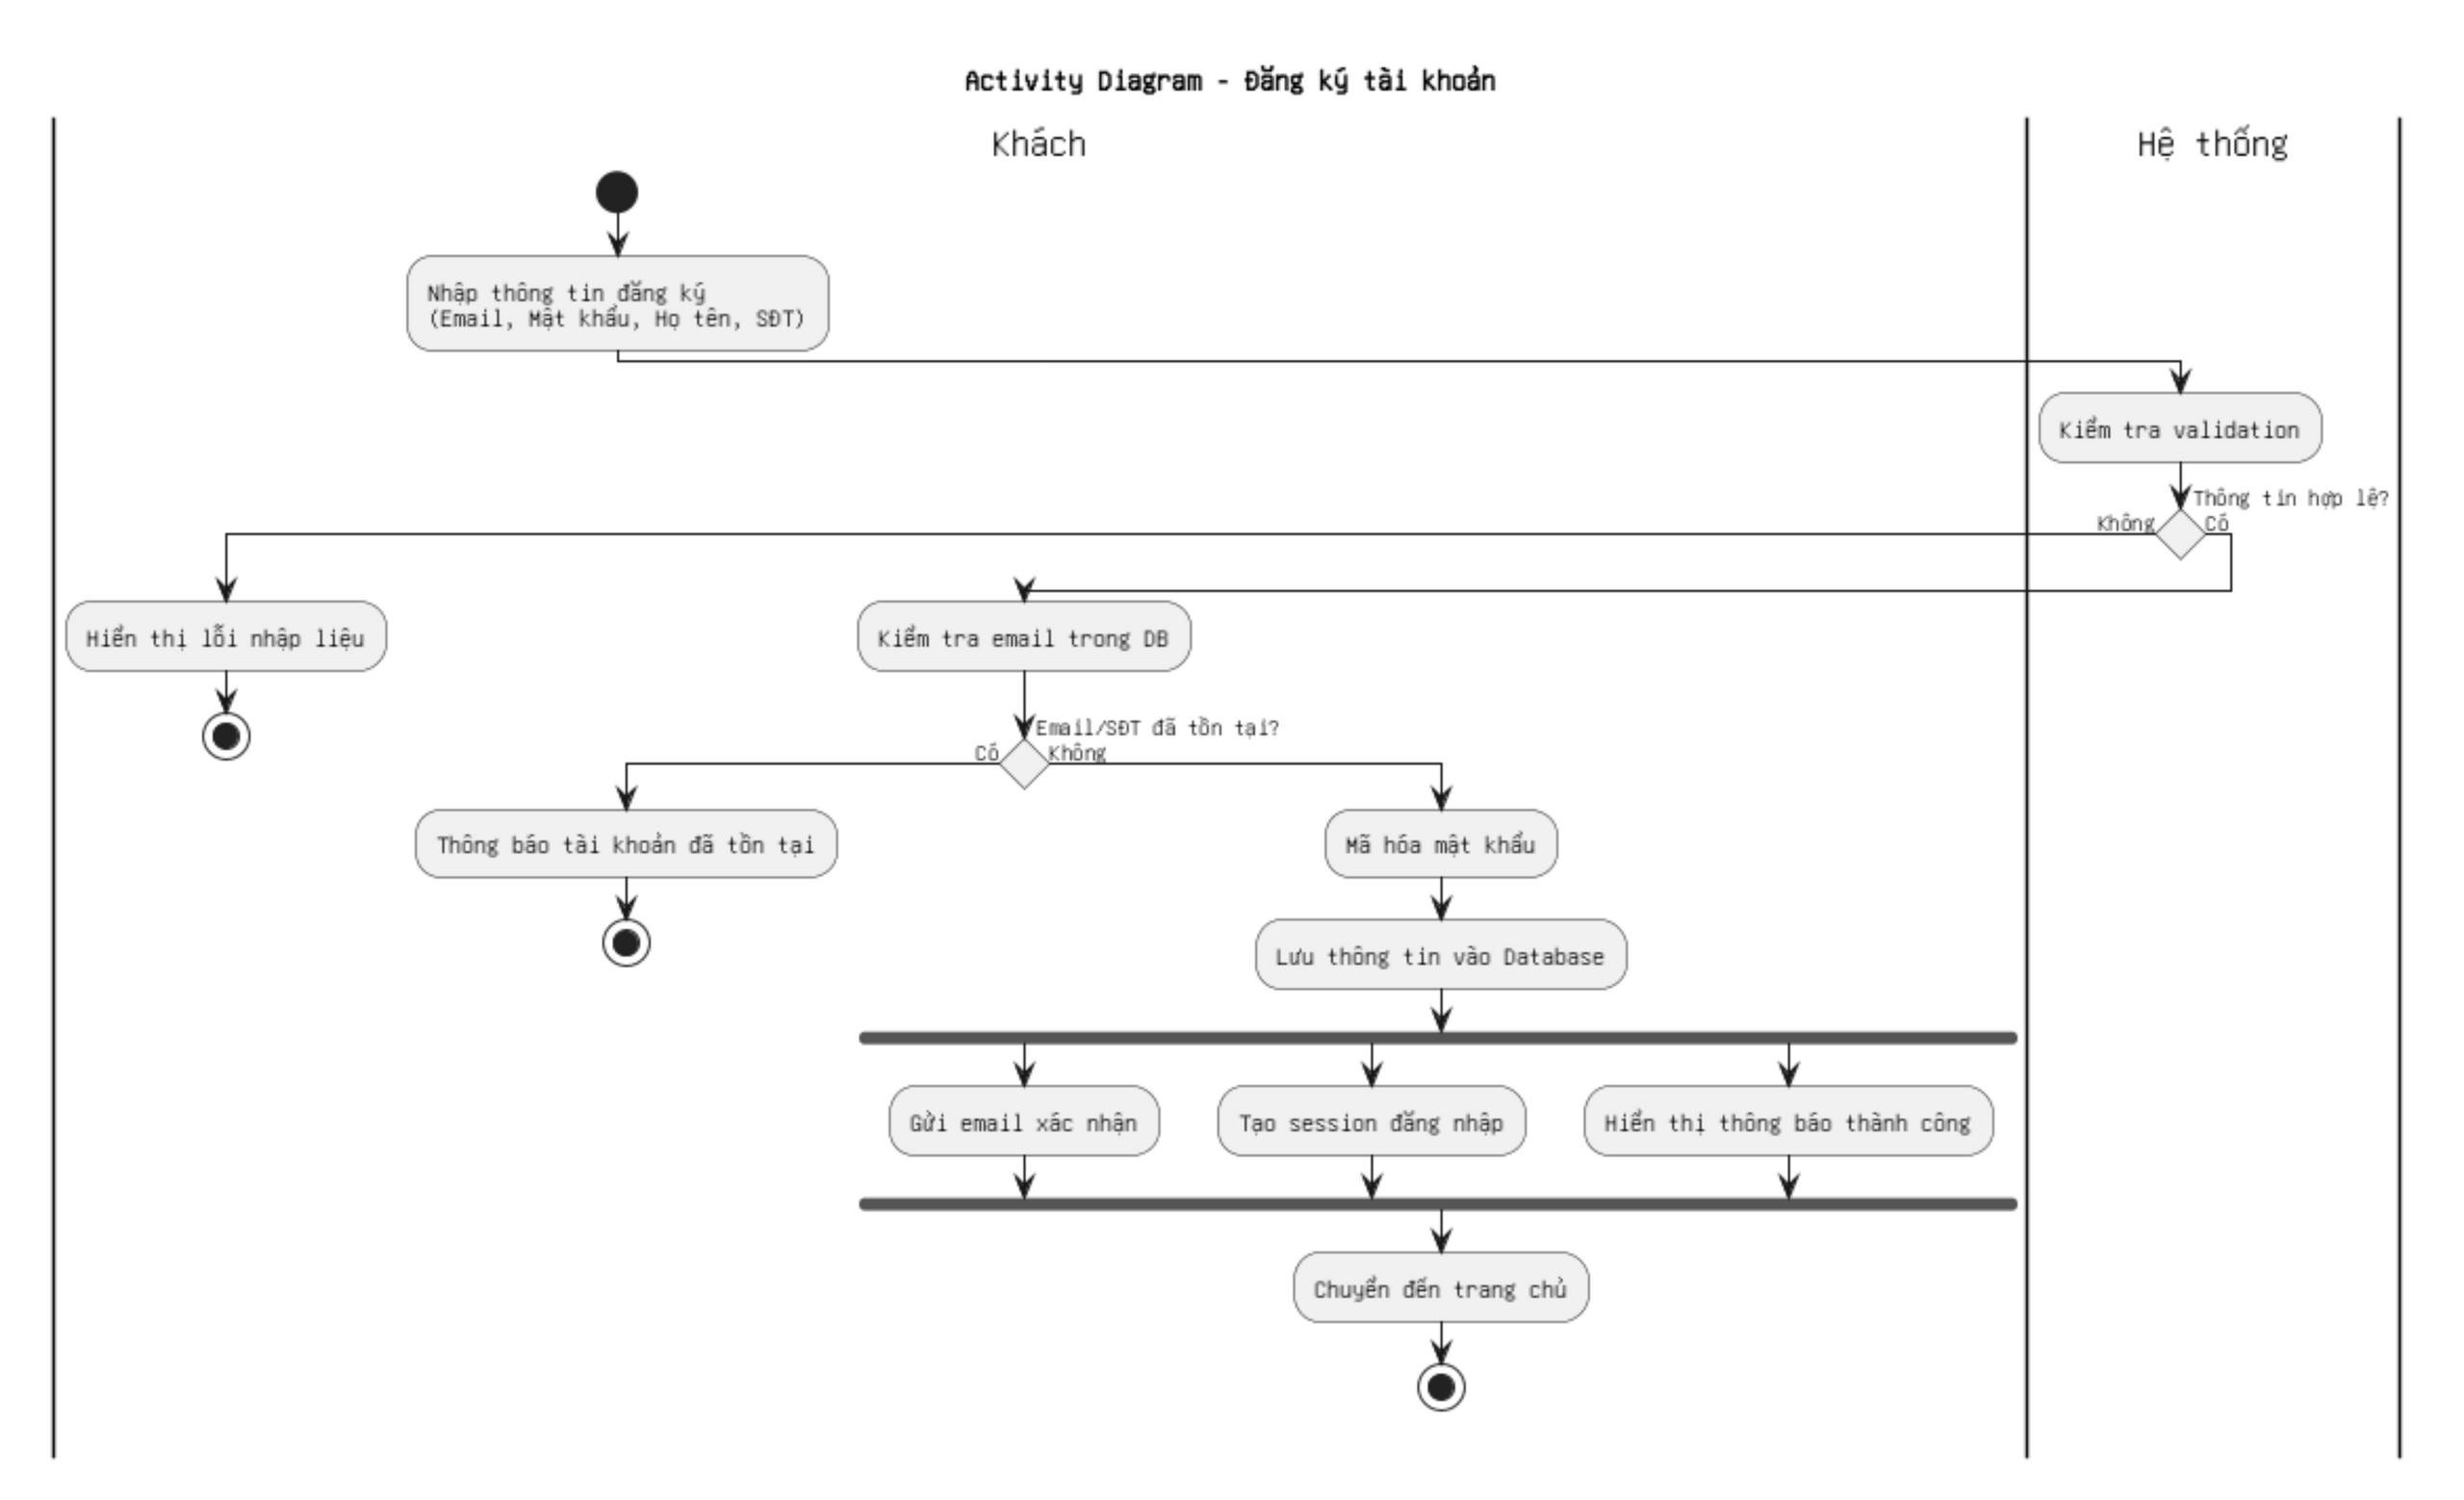
\includegraphics[width=0.7\textwidth]{figures/ac_dk.jpg}
    \caption{Activity Diagram xử lý đăng ký}
    \label{fig:ac_dk}
\end{figure}

\textbf{Mục đích:} Cho phép người dùng tạo tài khoản mới trong hệ thống bằng cách nhập thông tin cá nhân và xác thực qua email.

\textbf{Luồng hoạt động:}

\begin{itemize}
    \item Khách hàng nhập thông tin đăng ký (Email, Mật khẩu, Họ tên).
    \item Hệ thống kiểm tra validation thông tin:
    \begin{itemize}
        \item \textit{Nếu không hợp lệ:} Hiển thị lỗi nhập liệu và kết thúc.
        \item \textit{Nếu hợp lệ:} Tiếp tục kiểm tra email trong database.
    \end{itemize}
    \item Hệ thống kiểm tra email đã tồn tại:
    \begin{itemize}
        \item \textit{Nếu đã tồn tại:} Thông báo tài khoản đã tồn tại và kết thúc.
        \item \textit{Nếu chưa tồn tại:} Mã hóa mật khẩu và lưu thông tin vào database.
    \end{itemize}
    \item Hệ thống thực hiện song song:
    \begin{itemize}
        \item Gửi email xác nhận
        \item Tạo session đăng nhập
        \item Hiển thị thông báo thành công
    \end{itemize}
    \item Chuyển đến trang chủ và kết thúc quy trình.
\end{itemize}



\subsection{Activity Diagram xử lý đăng nhập}
\begin{figure}[H]
    \centering
    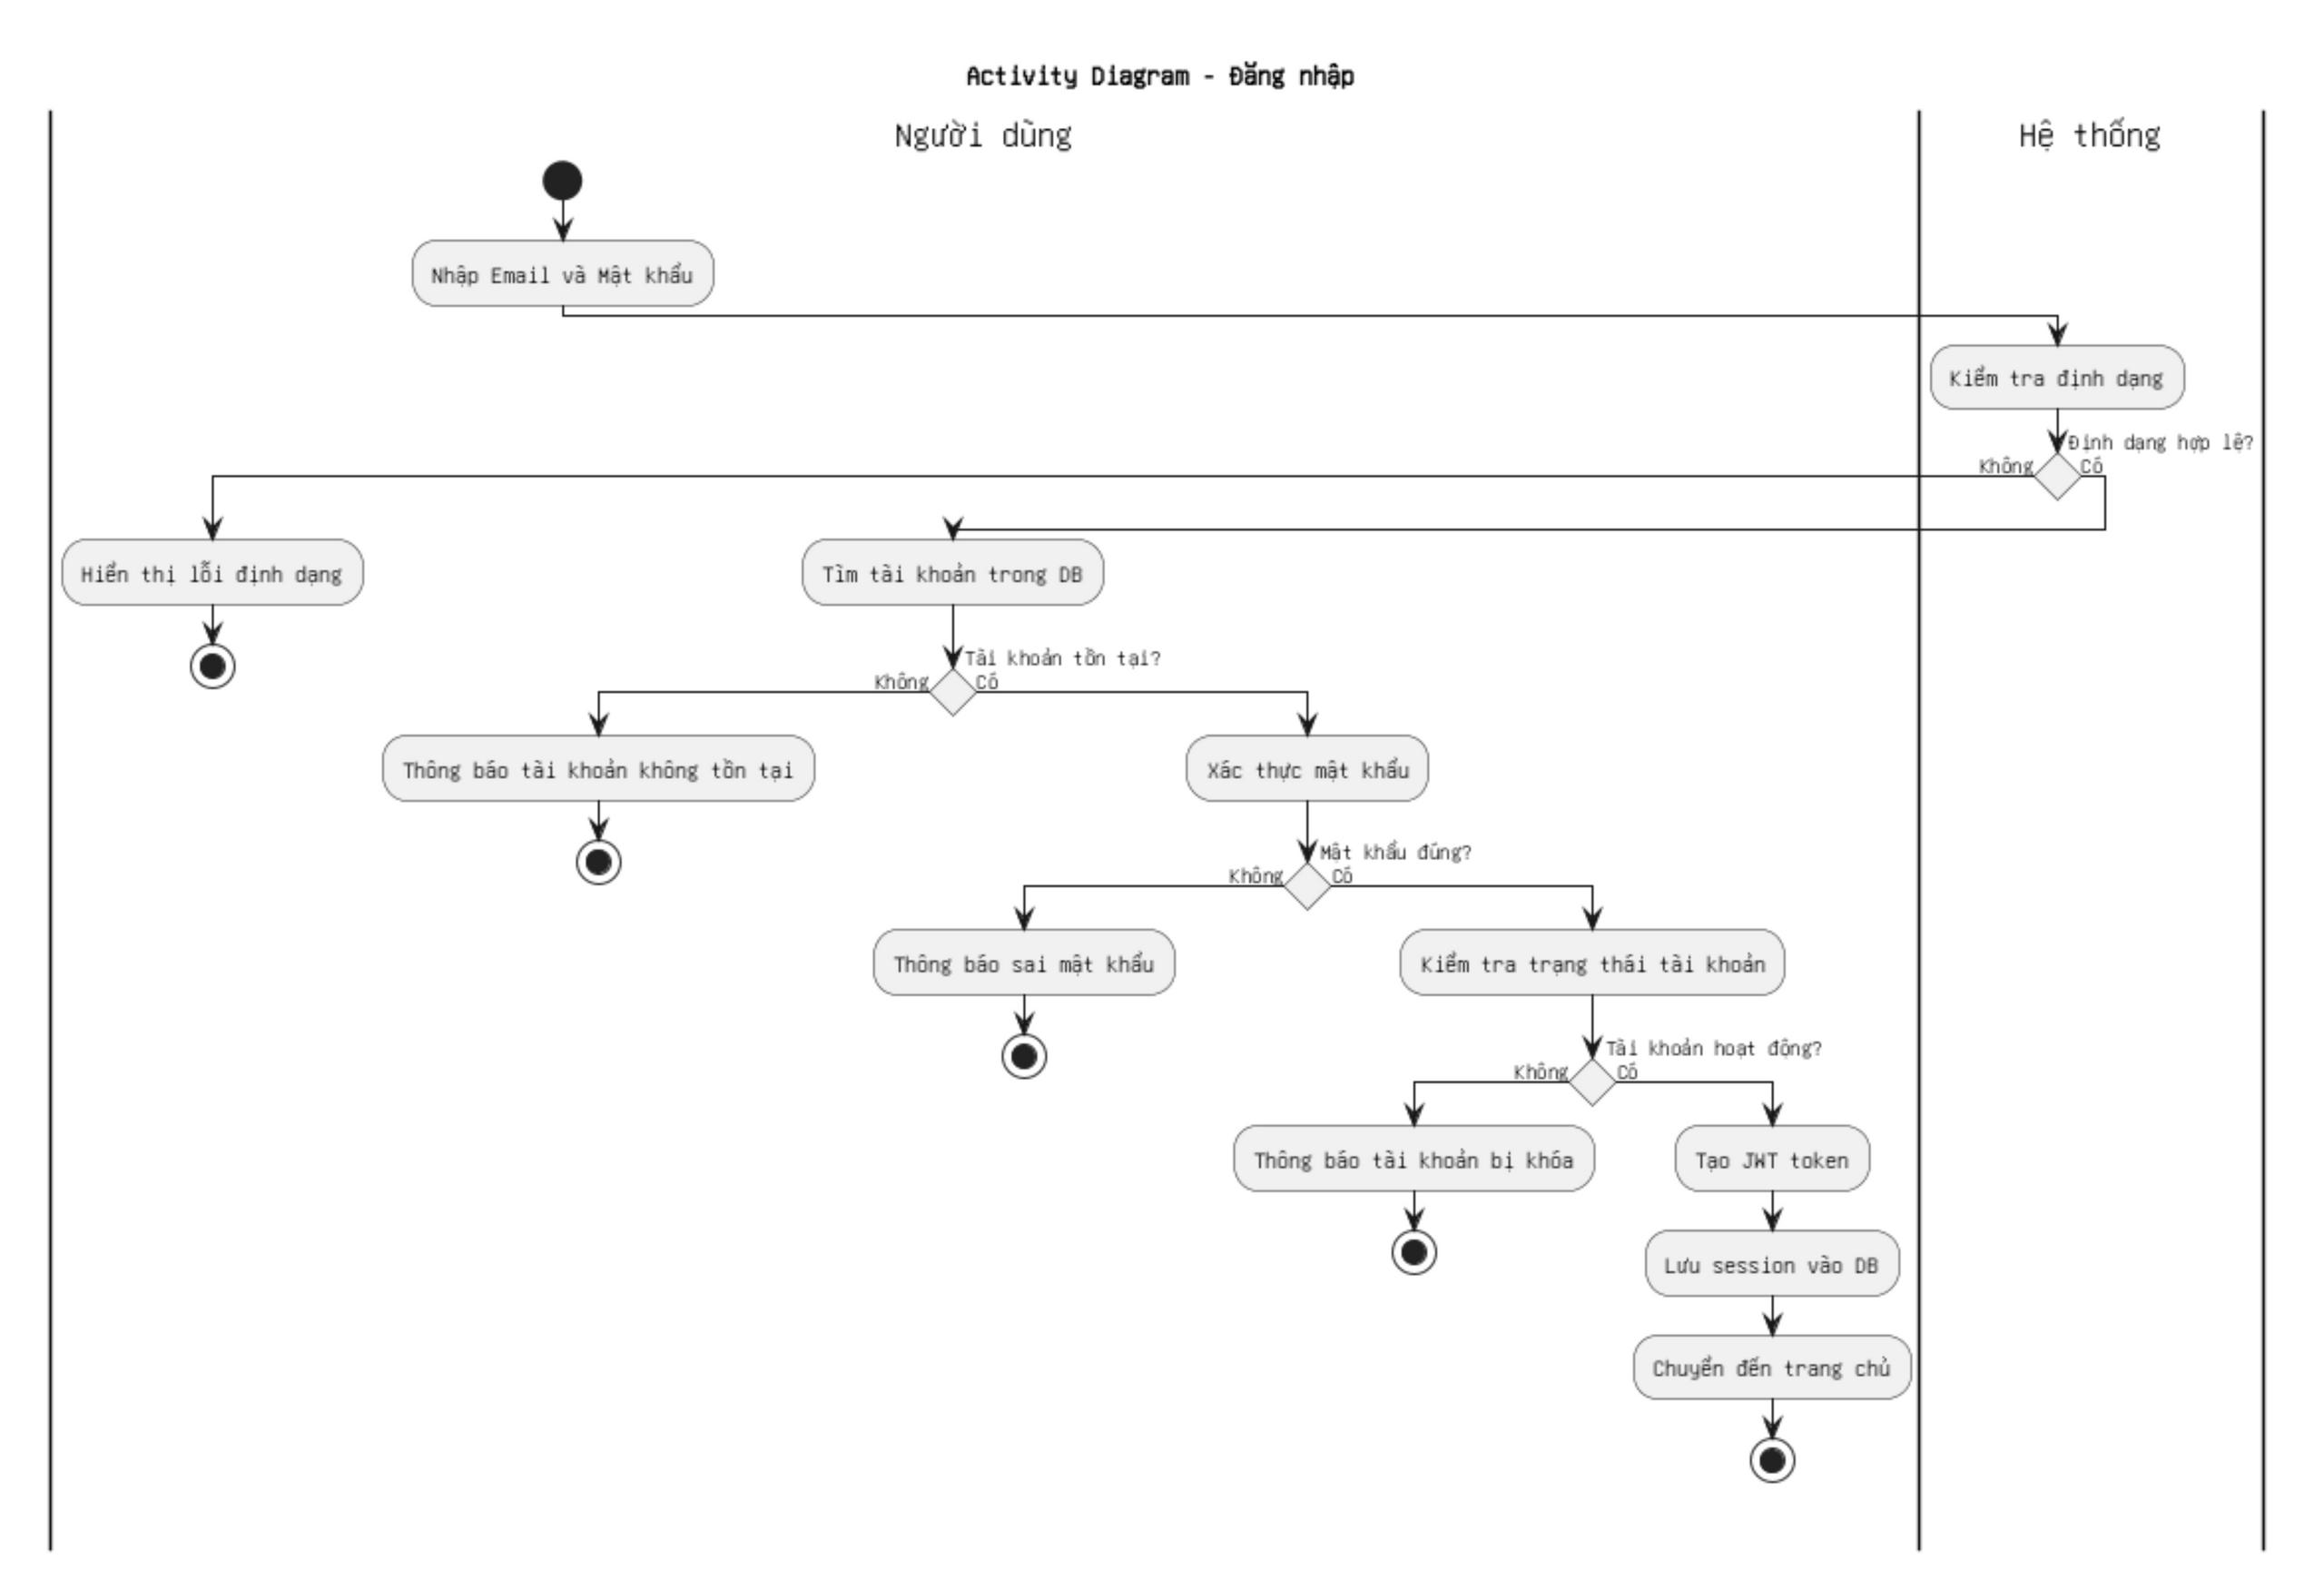
\includegraphics[width=0.7\textwidth]{figures/ac_dn.jpg}
    \caption{Activity Diagram xử lý đăng nhập}
    \label{fig:ac_dn}
\end{figure}
\textbf{Mục đích:} Cho phép người dùng xác thực và truy cập vào hệ thống bằng tài khoản đã đăng ký.

\textbf{Luồng hoạt động:}

\begin{itemize}
    \item Người dùng nhập Email và Mật khẩu.
    \item Hệ thống kiểm tra định dạng:
    \begin{itemize}
        \item \textit{Nếu không hợp lệ:} Hiển thị lỗi định dạng và kết thúc.
        \item \textit{Nếu hợp lệ:} Tìm tài khoản trong database.
    \end{itemize}
    \item Hệ thống kiểm tra tài khoản tồn tại:
    \begin{itemize}
        \item \textit{Nếu không tồn tại:} Thông báo tài khoản không tồn tại và kết thúc.
        \item \textit{Nếu tồn tại:} Xác thực mật khẩu.
    \end{itemize}
    \item Hệ thống xác thực mật khẩu:
    \begin{itemize}
        \item \textit{Nếu sai:} Thông báo sai mật khẩu và kết thúc.
        \item \textit{Nếu đúng:} Kiểm tra trạng thái tài khoản.
    \end{itemize}
    \item Hệ thống kiểm tra tài khoản hoạt động:
    \begin{itemize}
        \item \textit{Nếu bị khóa:} Thông báo tài khoản bị khóa và kết thúc.
        \item \textit{Nếu hoạt động:} Tạo JWT token.
    \end{itemize}
    \item Lưu session vào database.
    \item Chuyển đến trang chủ và kết thúc quy trình.
\end{itemize}




\subsection{Activity Diagram xử lý đặt lịch}
\begin{figure}[H]
    \centering
    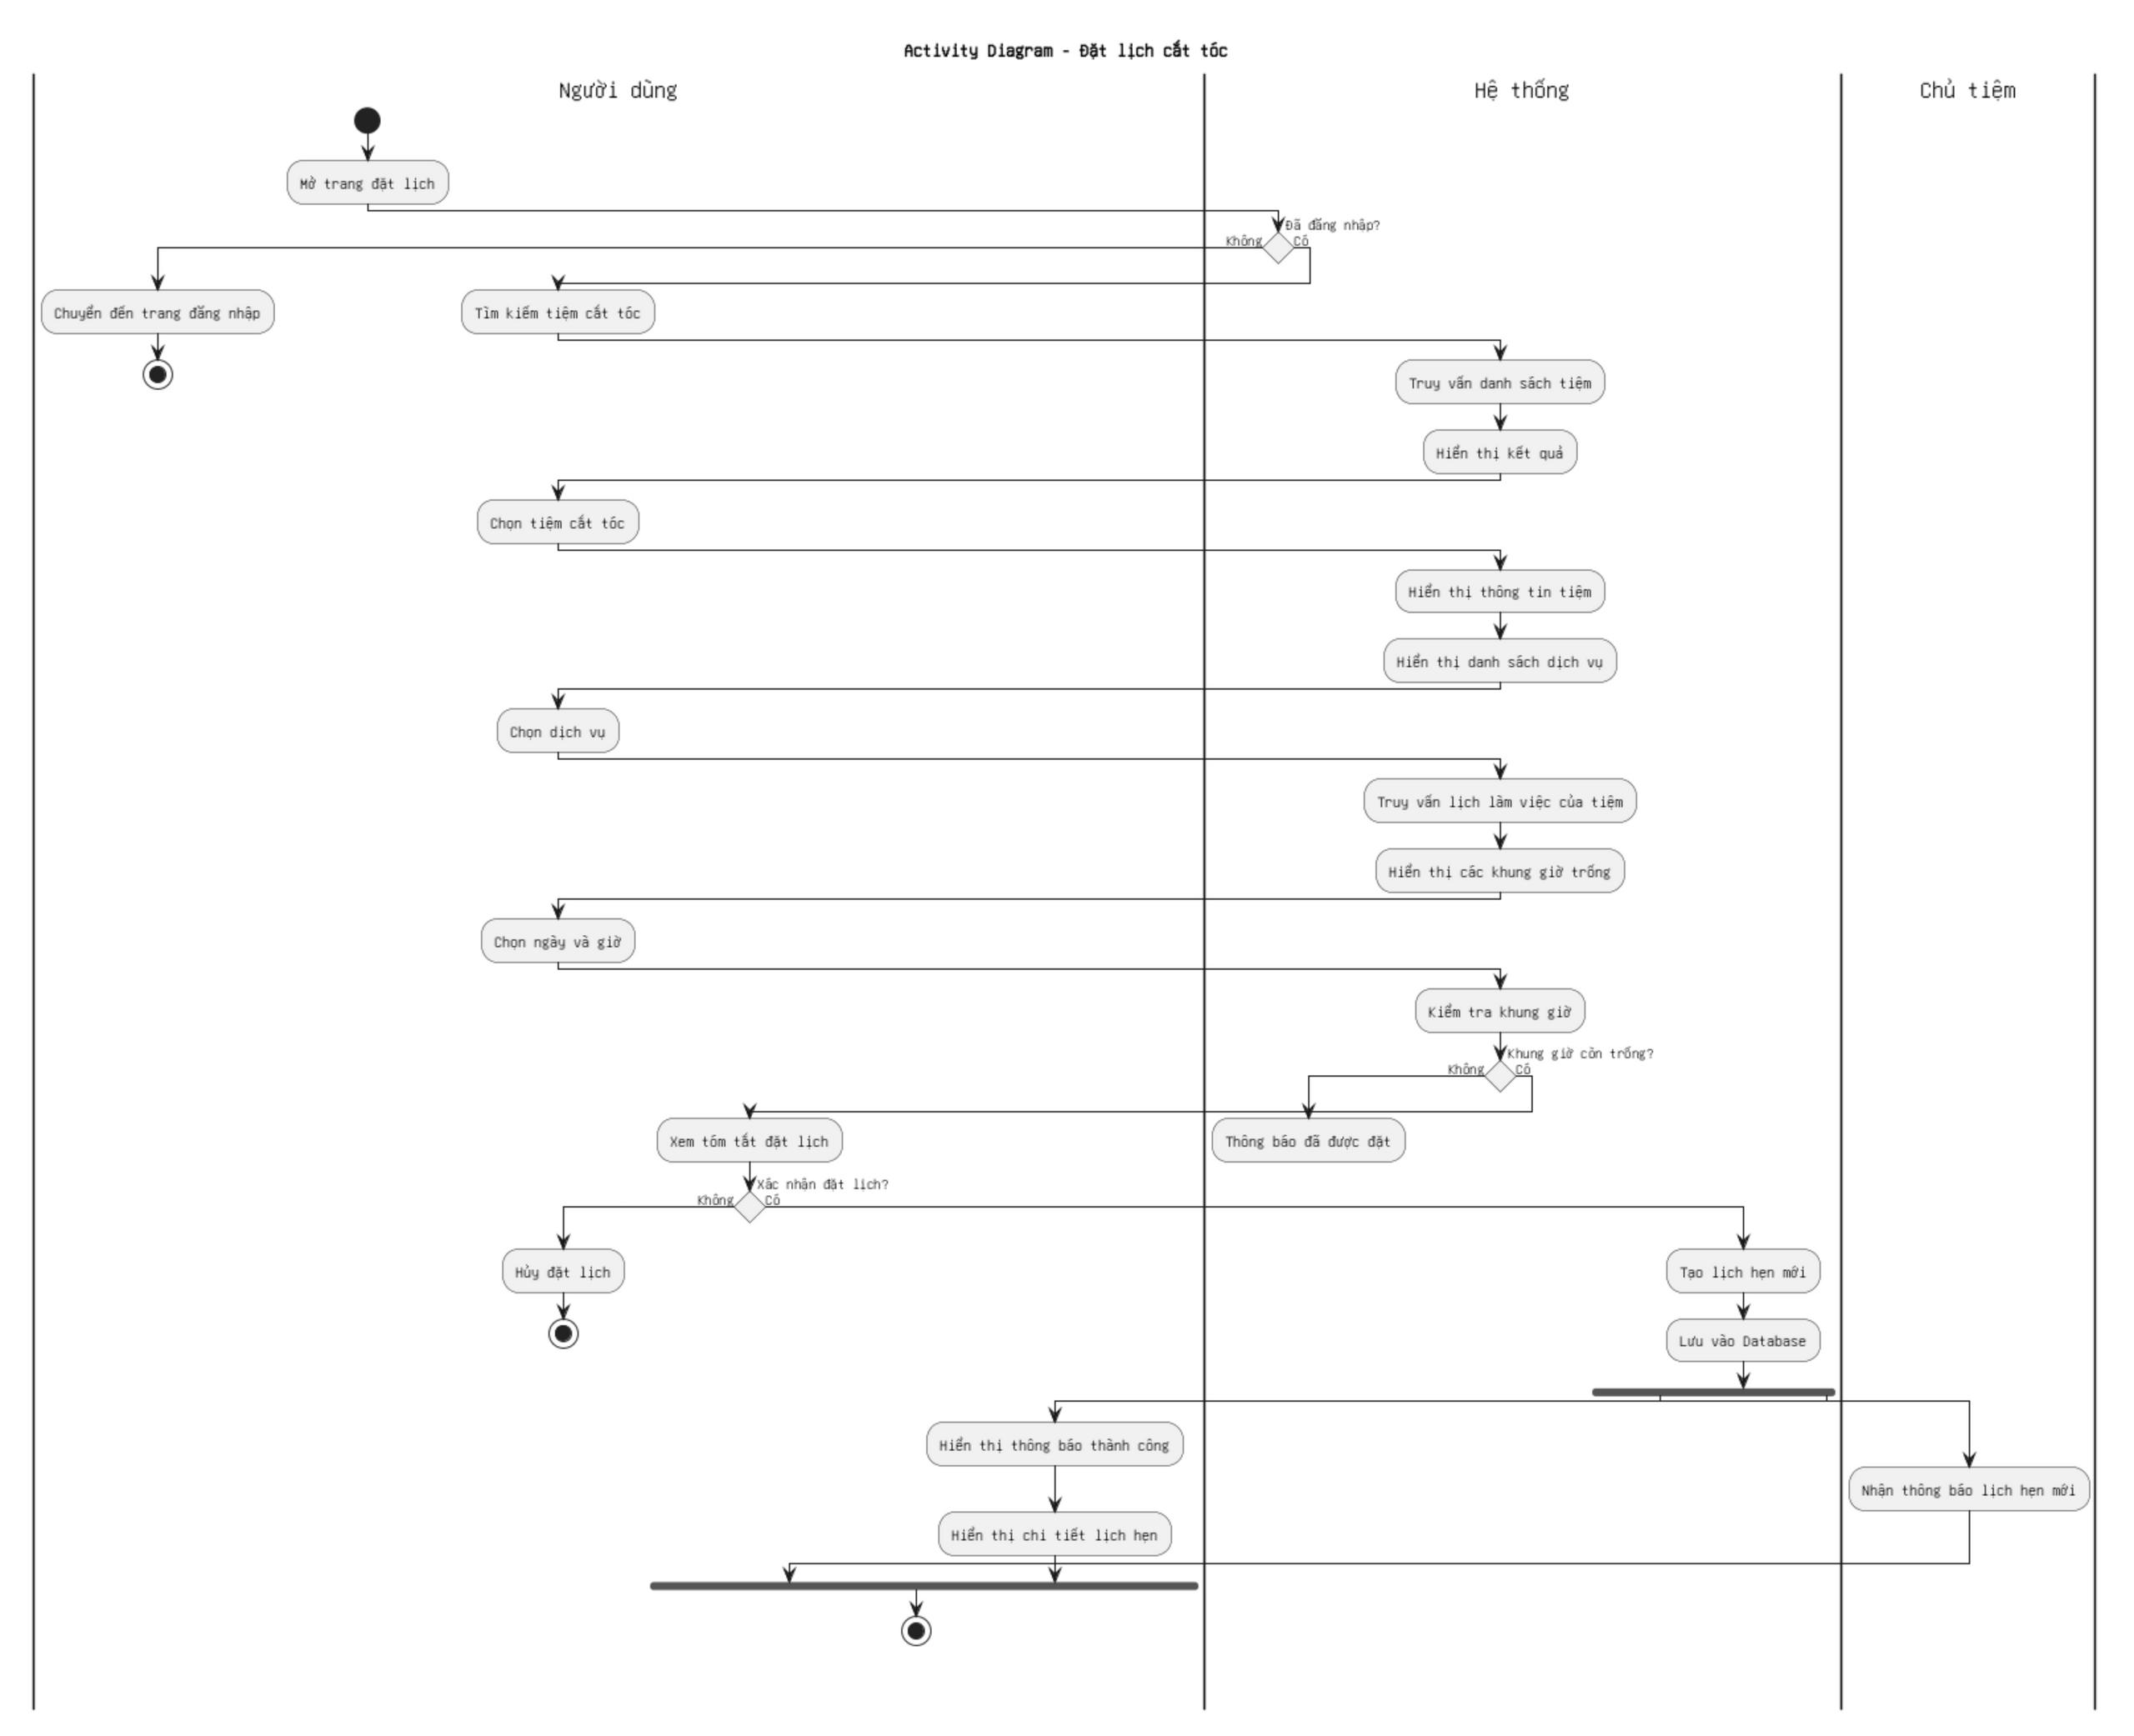
\includegraphics[width=0.7\textwidth]{figures/ac_booking.jpg}
    \caption{Activity Diagram xử lý đặt lịch}
    \label{fig:ac_booking}
\end{figure}

\textbf{Mục đích:} Cho phép người dùng đặt lịch hẹn cắt tóc tại tiệm bằng cách chọn thông tin liên quan và xác nhận đặt lịch.

\textbf{Luồng hoạt động:}

\begin{itemize}
    \item Người dùng mở trang đặt lịch.
    \item Hệ thống kiểm tra đăng nhập:
    \begin{itemize}
        \item \textit{Nếu chưa đăng nhập:} Chuyển đến trang đăng nhập và kết thúc.
        \item \textit{Nếu đã đăng nhập:} Tìm kiếm liên cắt tóc.
    \end{itemize}
    \item Chủ tiệm truy vấn danh sách tiệm và hiển thị kết quả.
    \item Người dùng chọn liệm cắt tóc, hệ thống hiển thị thông tin tiệm và kiểm tra danh sách dịch vụ.
    \item Người dùng chọn dịch vụ, hệ thống truy vấn liên lịch làm việc của tiệm và hiển thị các khung giờ trống.
    \item Người dùng chọn ngày và giờ, hệ thống kiểm tra khung giờ:
    \begin{itemize}
        \item \textit{Nếu khung giờ còn trống:} Thông báo đã được đặt.
        \item \textit{Nếu khung giờ đã hết:} Chờ người dùng chọn lại.
    \end{itemize}
    \item Người dùng xem tóm tắt đặt lịch và xác nhận đặt lịch:
    \begin{itemize}
        \item \textit{Nếu có nhận đặt lịch:} Hủy đặt lịch và kết thúc.
        \item \textit{Nếu xác nhận:} 
        \begin{itemize}
            \item Chủ tiệm tạo lịch hẹn mới và lưu vào database.
            \item Gửi thông báo lịch hẹn mới.
        \end{itemize}
    \end{itemize}
    \item Hiển thị thông báo thành công và chi tiết lịch hẹn.
    \item Kết thúc quy trình.
\end{itemize}


\subsection{Activity Diagram xử lý AI gợi ý kiểu tóc}
\begin{figure}[H]
    \centering
    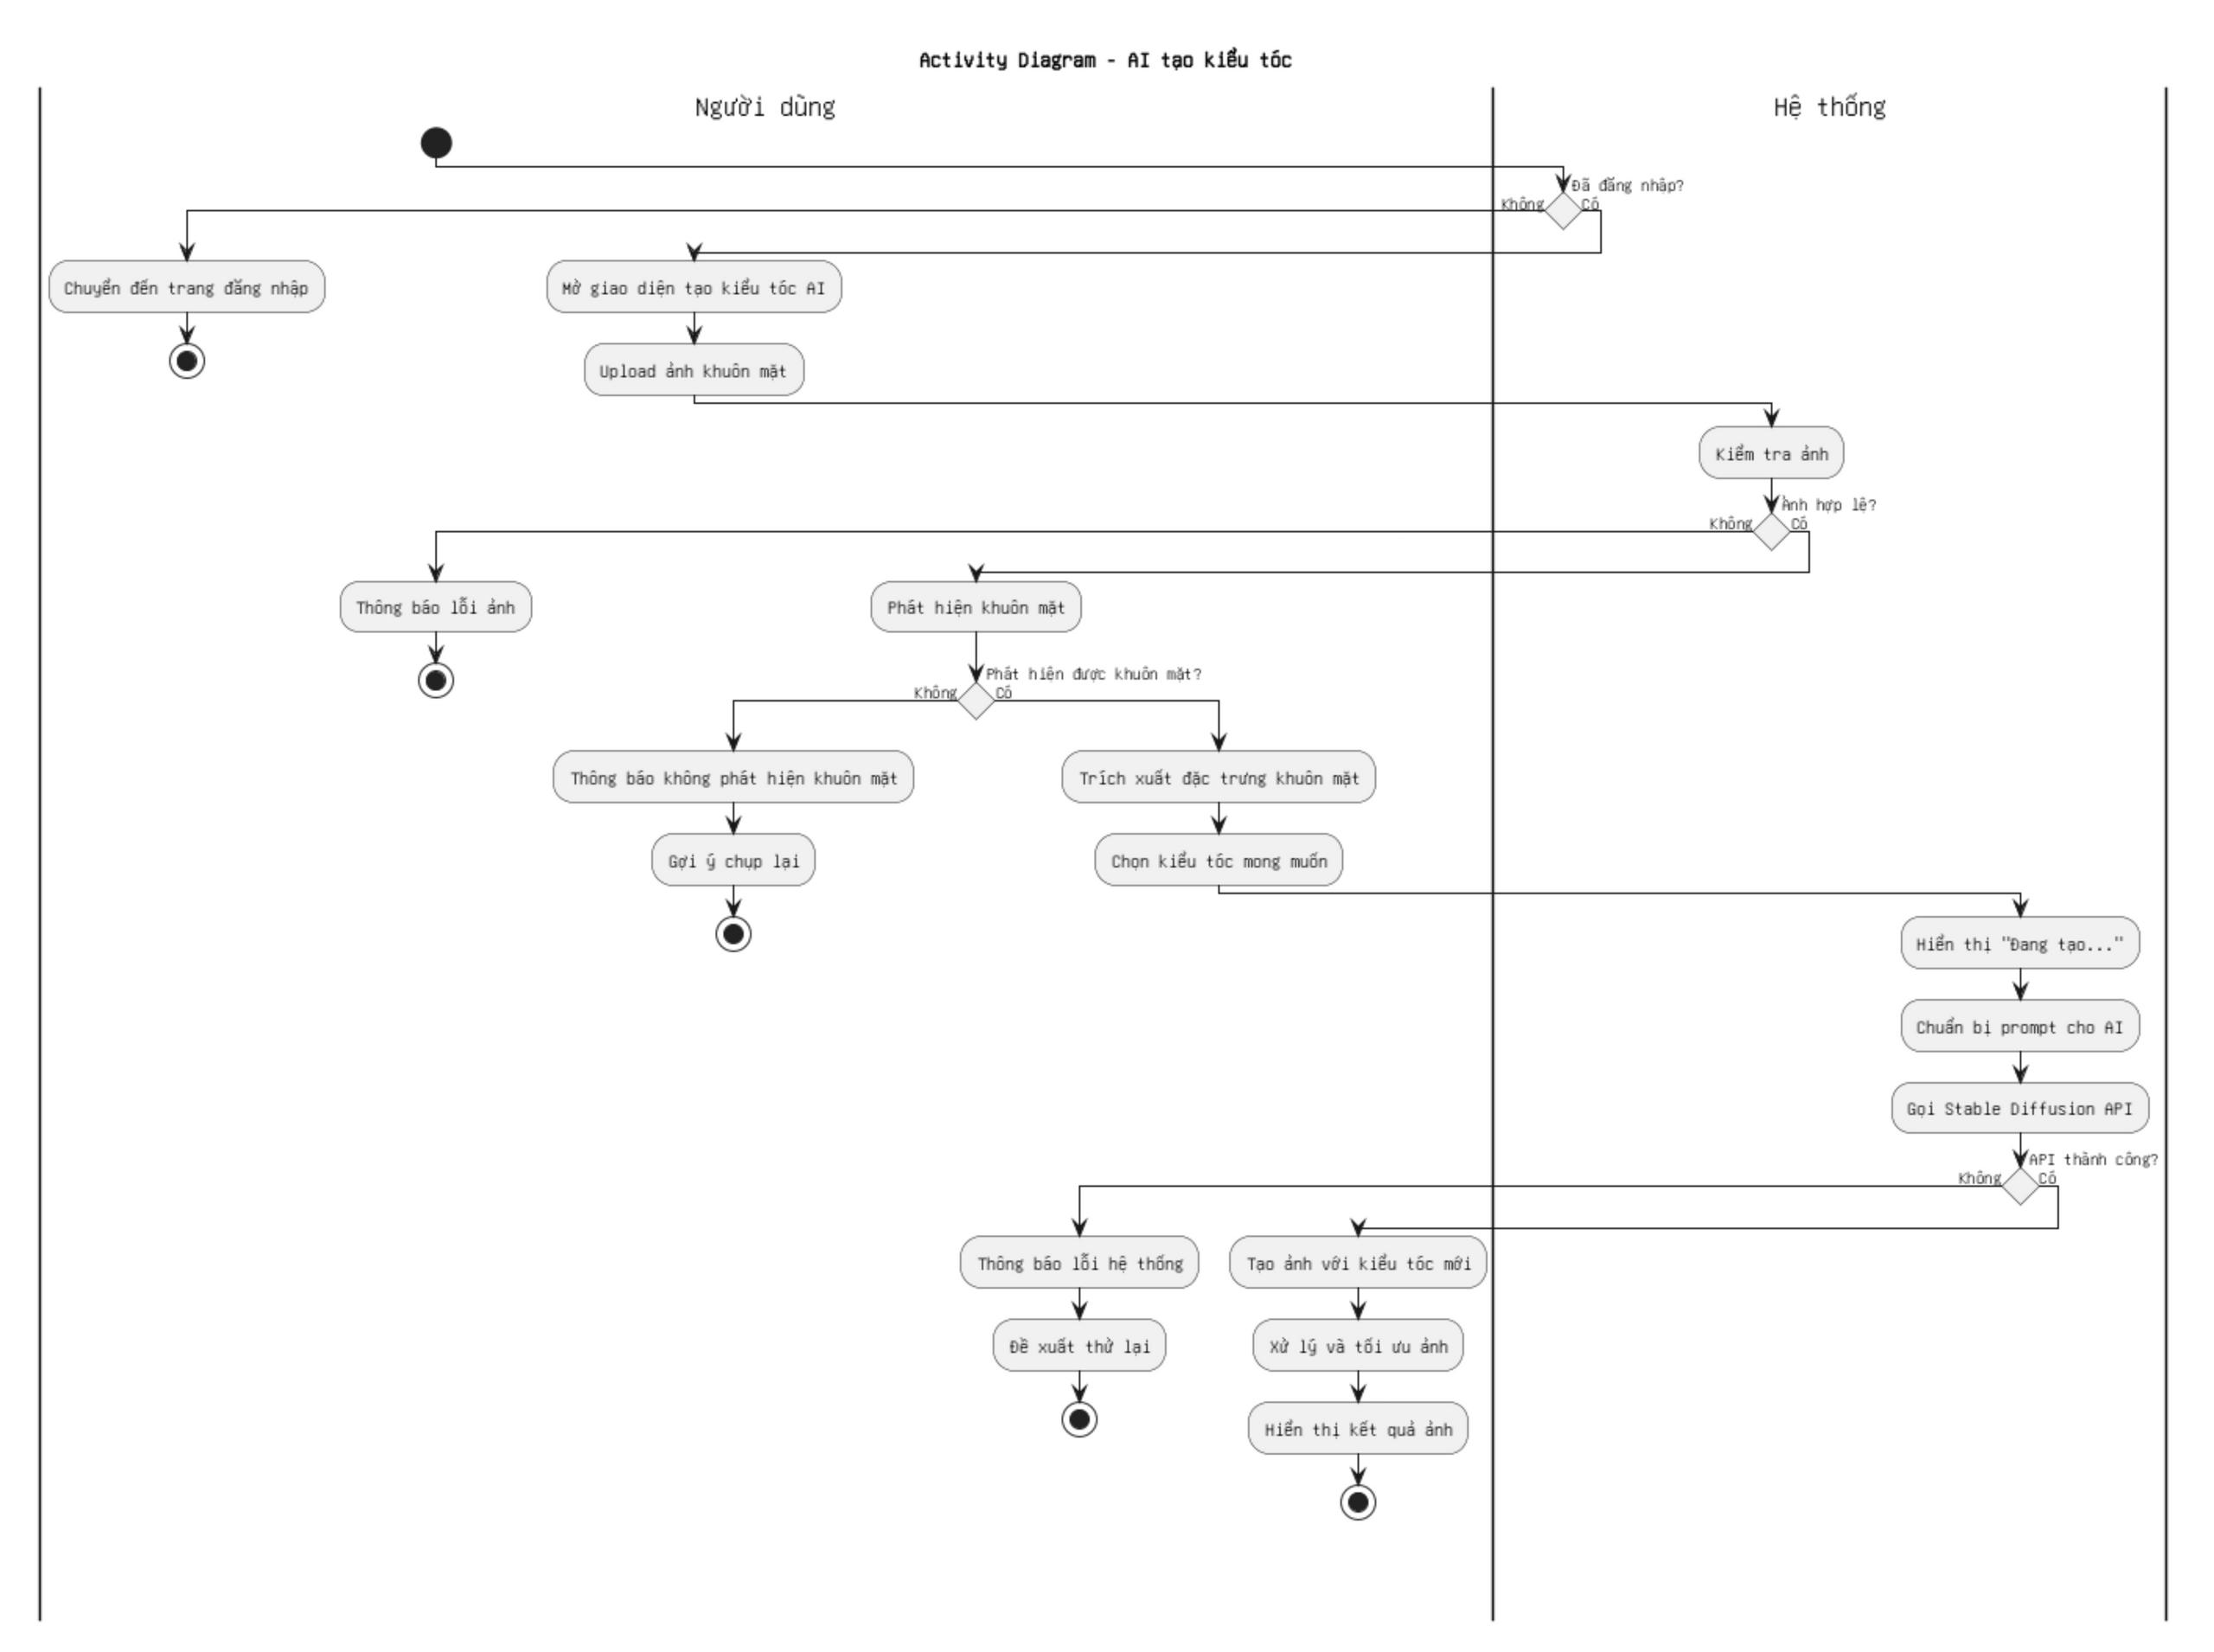
\includegraphics[width=0.8\textwidth]{figures/ac_hair.jpg}
    \caption{Activity Diagram xử lý AI gợi ý kiểu tóc}
    \label{fig:ac_hair}
\end{figure}

\textbf{Mục đích:} Cho phép người dùng sử dụng AI để tạo và xem trước kiểu tóc mong muốn từ ảnh khuôn mặt.

\textbf{Luồng hoạt động:}

\begin{itemize}
    \item Hệ thống kiểm tra đăng nhập:
    \begin{itemize}
        \item \textit{Nếu chưa đăng nhập:} Chuyển đến trang đăng nhập và kết thúc.
        \item \textit{Nếu đã đăng nhập:} Mở giao diện tạo kiểu tóc AI.
    \end{itemize}
    \item Người dùng upload ảnh khuôn mặt.
    \item Hệ thống kiểm tra định dạng ảnh:
    \begin{itemize}
        \item \textit{Nếu không hợp lệ:} Thông báo lỗi ảnh và kết thúc.
        \item \textit{Nếu hợp lệ:} Phát hiện khuôn mặt.
    \end{itemize}
    \item Hệ thống phát hiện được khuôn mặt:
    \begin{itemize}
        \item \textit{Nếu không:} Thông báo không phát hiện khuôn mặt, gửi ý chụp lại và kết thúc.
        \item \textit{Nếu có:} Trích xuất đặc trưng khuôn mặt và chọn kiểu tóc mong muốn.
    \end{itemize}
    \item Hệ thống:
    \begin{itemize}
        \item Hiển thị "Đang tạo..."
        \item Chuẩn bị prompt cho AI
        \item Gọi Stable Diffusion API
    \end{itemize}
    \item Kiểm tra API thành công:
    \begin{itemize}
        \item \textit{Nếu không:} Thông báo lỗi hệ thống, đề xuất thử lại và kết thúc.
        \item \textit{Nếu có:} Tạo ảnh với kiểu tóc mới, xử lý và tối ưu ảnh, hiển thị kết quả ảnh.
    \end{itemize}
    \item Kết thúc quy trình.
\end{itemize}

\subsection{Activity Diagram xử lý AI kiểm tra da mặt}
\begin{figure}[H]
    \centering
    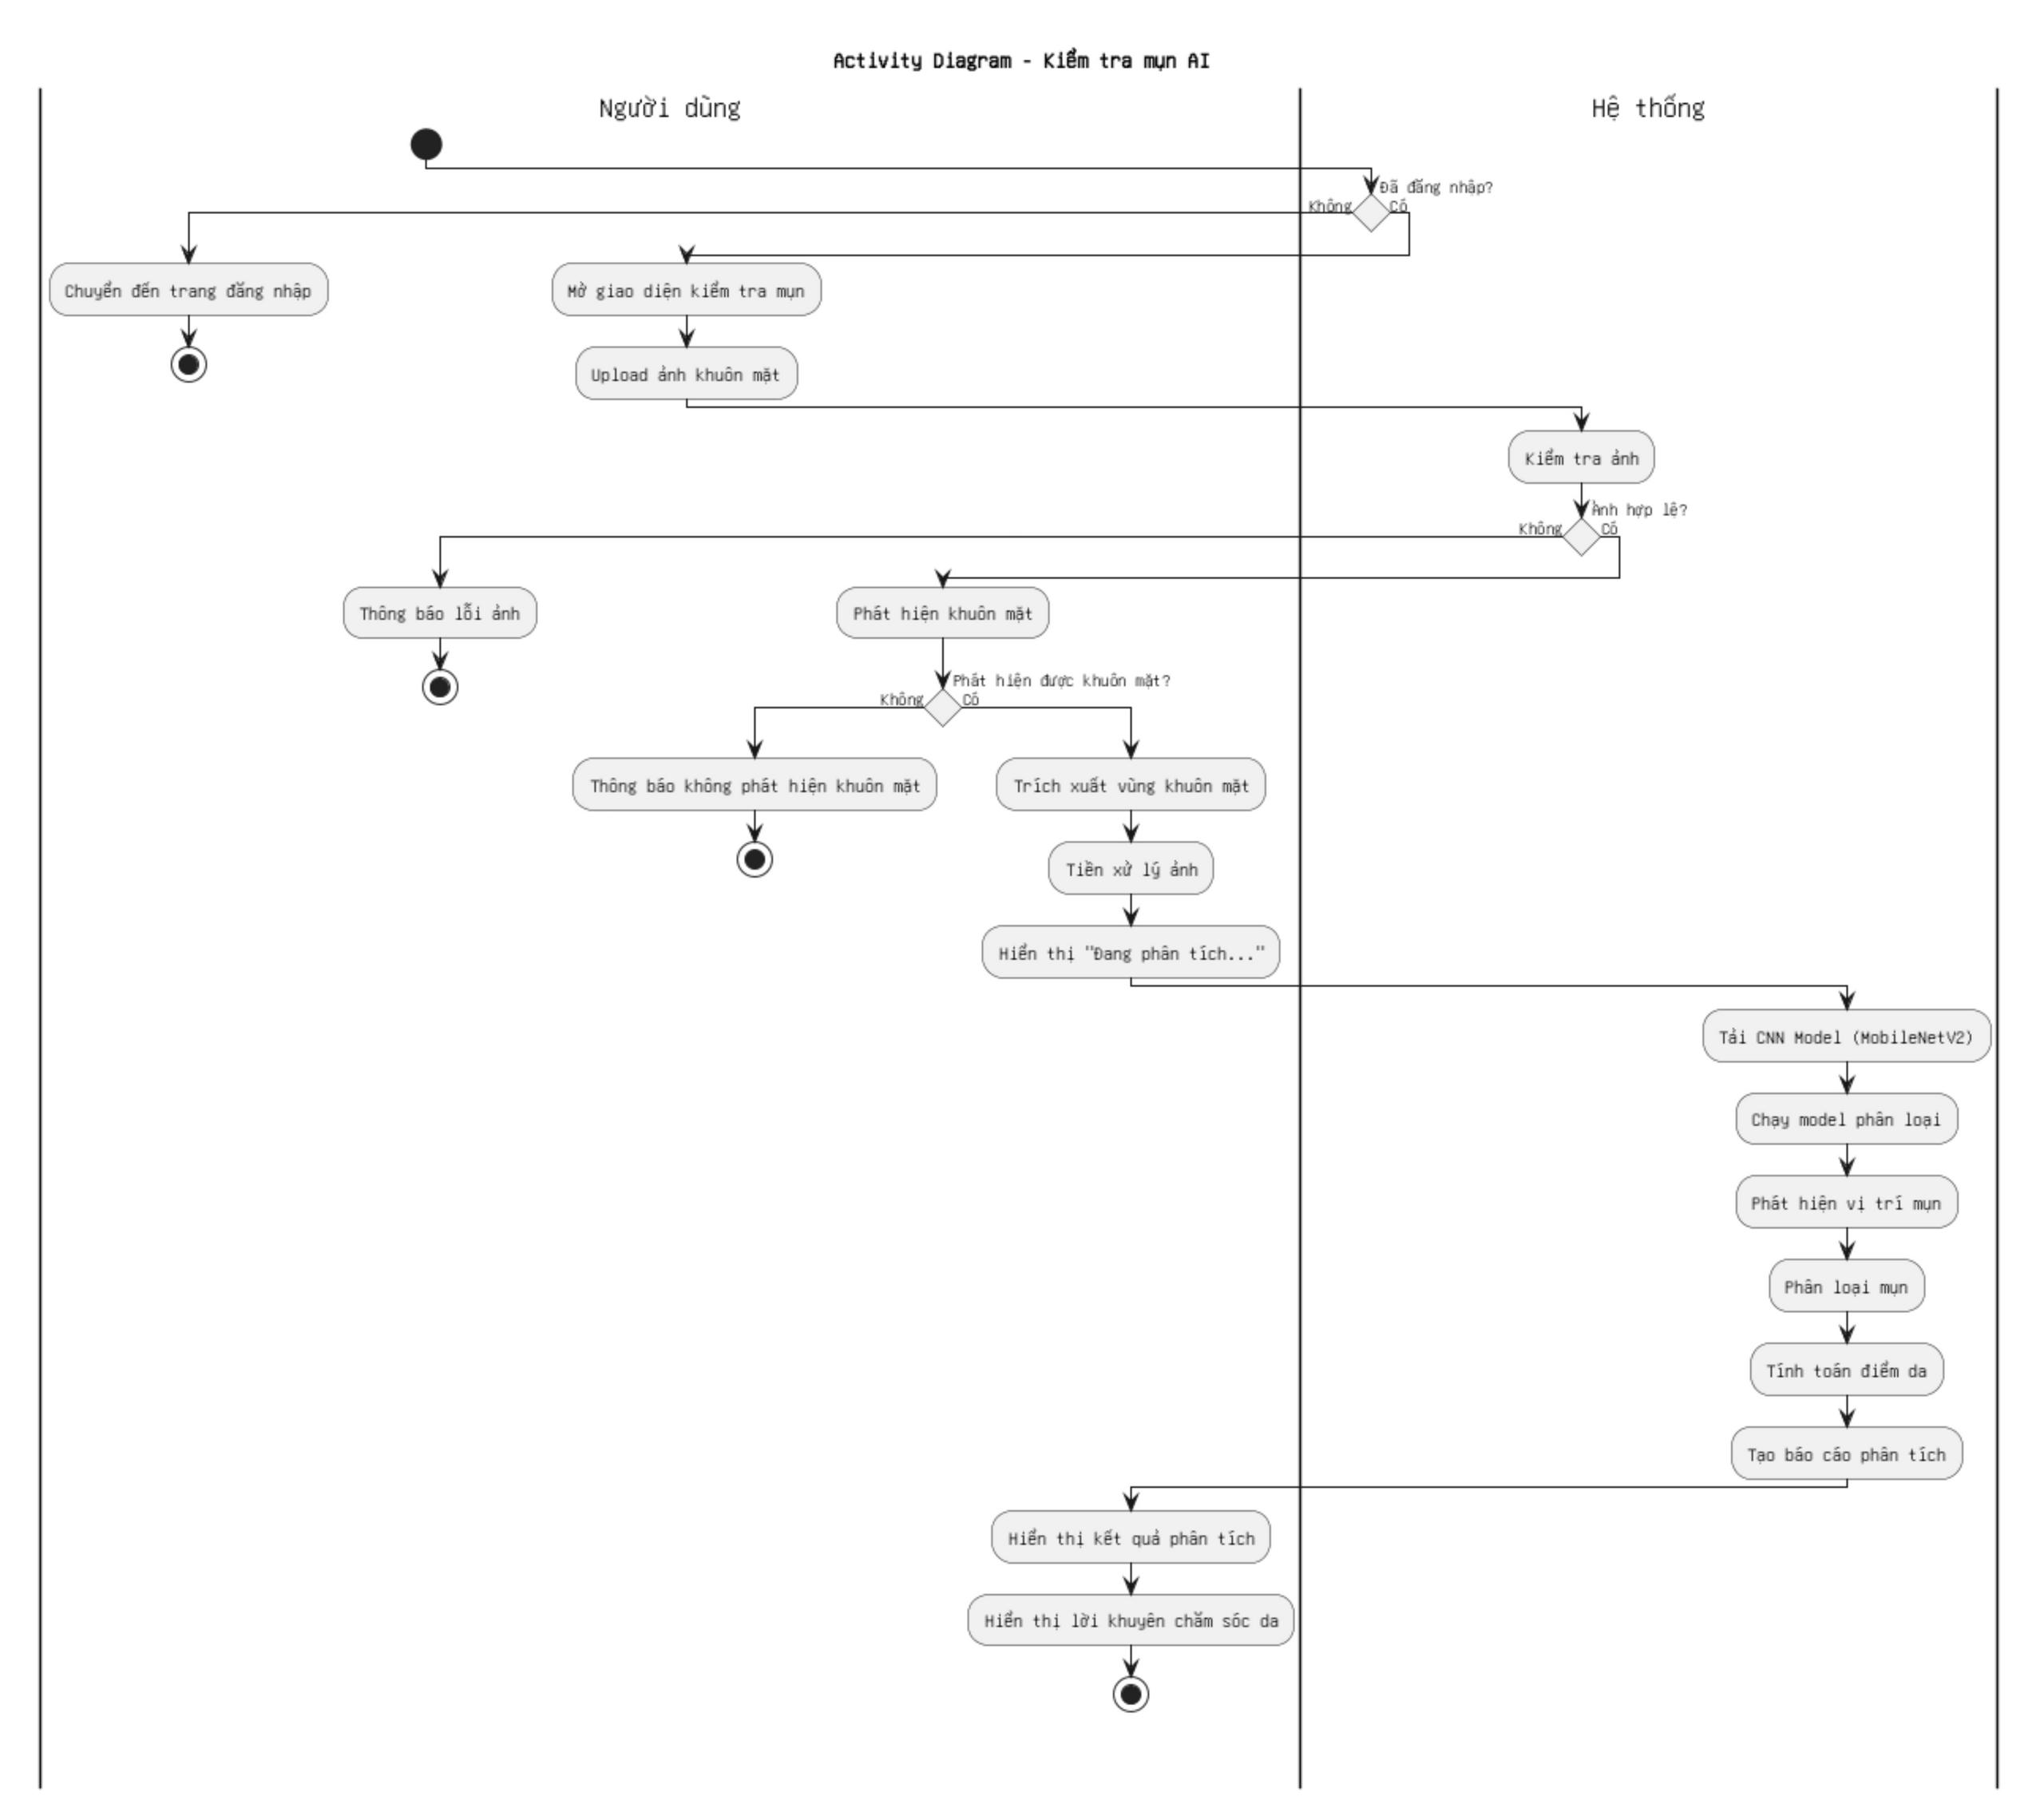
\includegraphics[width=0.8\textwidth]{figures/ac_mun.jpg}
    \caption{Activity Diagram xử lý AI kiểm tra da mặt}
    \label{fig:ac_mun}
\end{figure}


\textbf{Mục đích:} Cho phép người dùng sử dụng AI để phát hiện và phân tích tình trạng mụn trên khuôn mặt thông qua ảnh.

\textbf{Luồng hoạt động:}

\begin{itemize}
    \item Hệ thống kiểm tra đăng nhập:
    \begin{itemize}
        \item \textit{Nếu chưa đăng nhập:} Chuyển đến trang đăng nhập và kết thúc.
        \item \textit{Nếu đã đăng nhập:} Mở giao diện kiểm tra mụn.
    \end{itemize}
    \item Người dùng upload ảnh khuôn mặt.
    \item Hệ thống kiểm tra định dạng ảnh:
    \begin{itemize}
        \item \textit{Nếu không hợp lệ:} Thông báo lỗi ảnh và kết thúc.
        \item \textit{Nếu hợp lệ:} Phát hiện khuôn mặt.
    \end{itemize}
    \item Hệ thống phát hiện được khuôn mặt:
    \begin{itemize}
        \item \textit{Nếu không:} Thông báo không phát hiện khuôn mặt và kết thúc.
        \item \textit{Nếu có:} Trích xuất vùng khuôn mặt và tiền xử lý ảnh.
    \end{itemize}
    \item Hiển thị "Đang phân tích...".
    \item Hệ thống:
    \begin{itemize}
        \item Tải CNN Model (MobileNetV2)
        \item Chạy model phân loại
        \item Phát hiện vị trí mụn
        \item Phân loại mụn
        \item Tính toán điểm da
        \item Tạo báo cáo phân tích
    \end{itemize}
    \item Hiển thị kết quả phân tích.
    \item Hiển thị lời khuyên chăm sóc da.
    \item Kết thúc quy trình.
\end{itemize}

\subsection{Activity Diagram xử lý AI chatbot}
\begin{figure}[H]
    \centering
    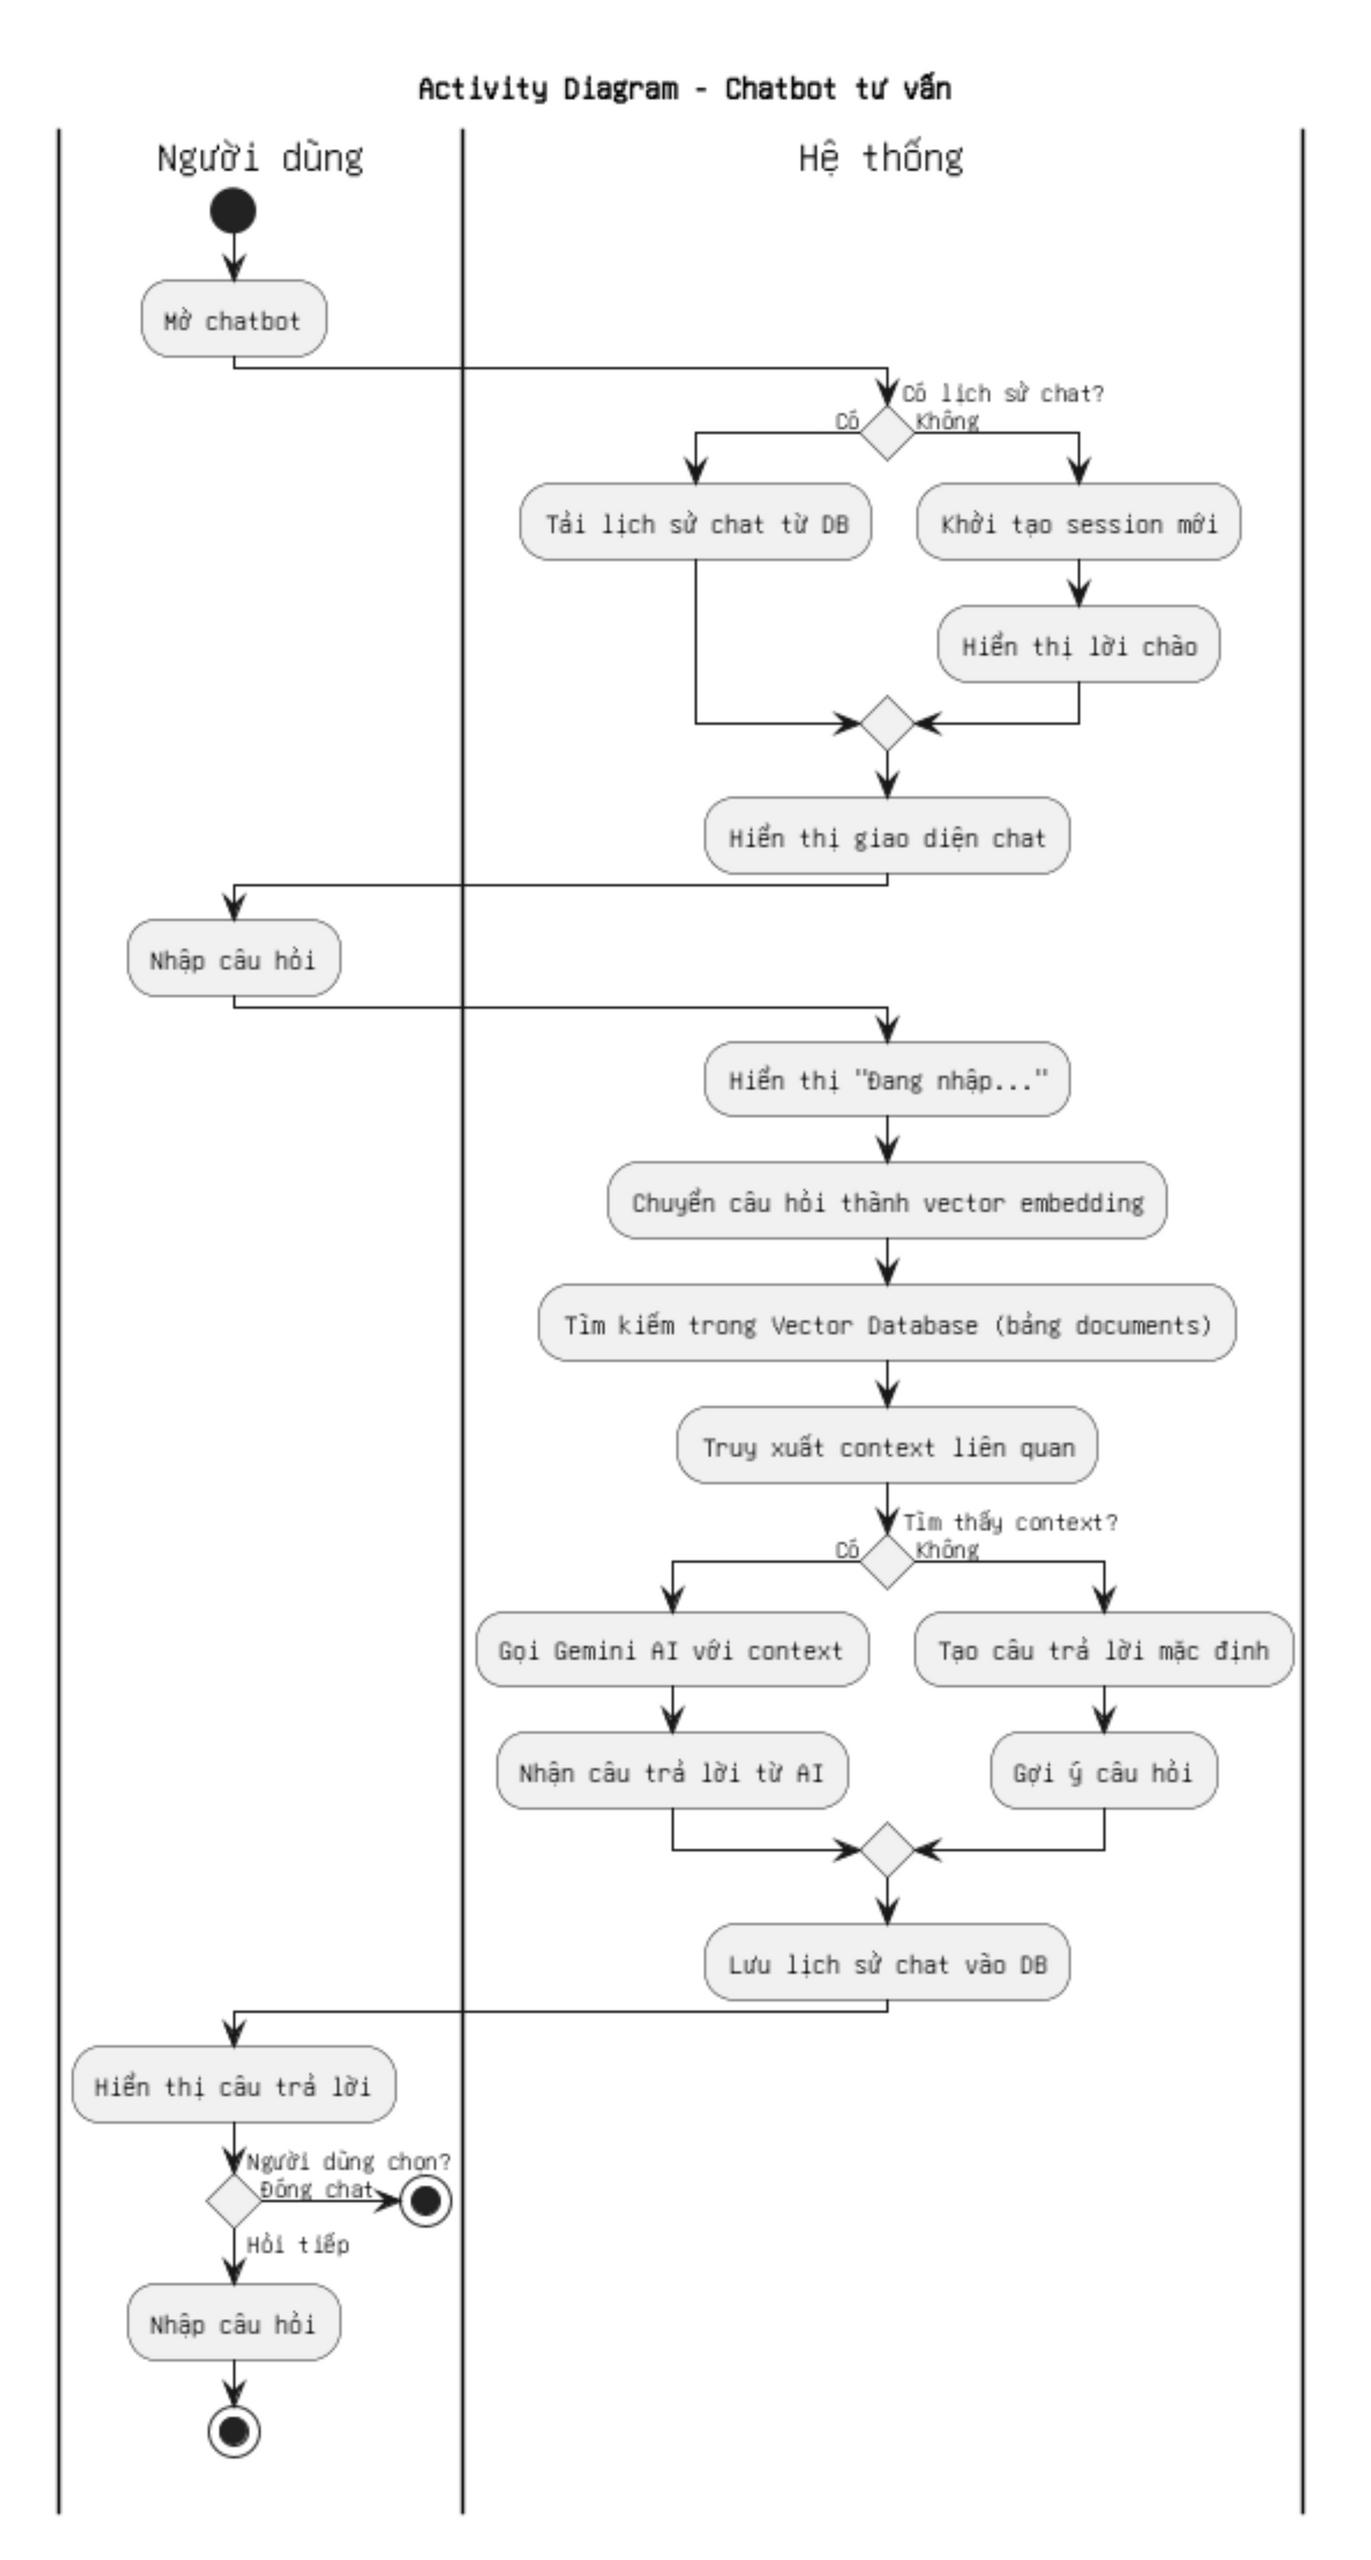
\includegraphics[width=0.5\textwidth]{figures/ac_tu_van.jpg}
    \caption{Activity Diagram xử lý AI chatbot}
    \label{fig:ac_chat}
\end{figure}

\textbf{Mục đích:} Cho phép người dùng tương tác với chatbot AI để được tư vấn về các dịch vụ cắt tóc, làm đẹp sử dụng công nghệ RAG (Retrieval-Augmented Generation).

\textbf{Luồng hoạt động:}

\begin{itemize}
    \item Người dùng mở chatbot.
    \item Hệ thống kiểm tra lịch sử chat:
    \begin{itemize}
        \item \textit{Nếu chưa có:} Tải lịch sử chat từ database.
        \item \textit{Nếu có:} Khởi tạo session mới và hiển thị lời chào.
    \end{itemize}
    \item Hiển thị giao diện chat.
    \item Người dùng nhập câu hỏi.
    \item Hệ thống hiển thị "Đang nhắp...".
    \item Chuyển câu hỏi thành vector embedding.
    \item Tìm kiếm trong Vector Database (bằng documents).
    \item Truy xuất context liên quan.
    \item Kiểm tra tìm thấy context:
    \begin{itemize}
        \item \textit{Nếu có:} Gọi Gemini AI với context.
        \item \textit{Nếu không:} Tạo câu trả lời mặc định.
    \end{itemize}
    \item Nhận câu trả lời từ AI và gửi ý câu hỏi.
    \item Lưu lịch sử chat vào database.
    \item Hiển thị câu trả lời.
    \item Kiểm tra người dùng chạy:
    \begin{itemize}
        \item \textit{Nếu chưa xong:} Quay lại bước nhập câu hỏi.
        \item \textit{Nếu xong:} Kết thúc quy trình.
    \end{itemize}
\end{itemize}



\subsection{Activity Diagram xử lý hợp tác}
\begin{figure}[H]
    \centering
    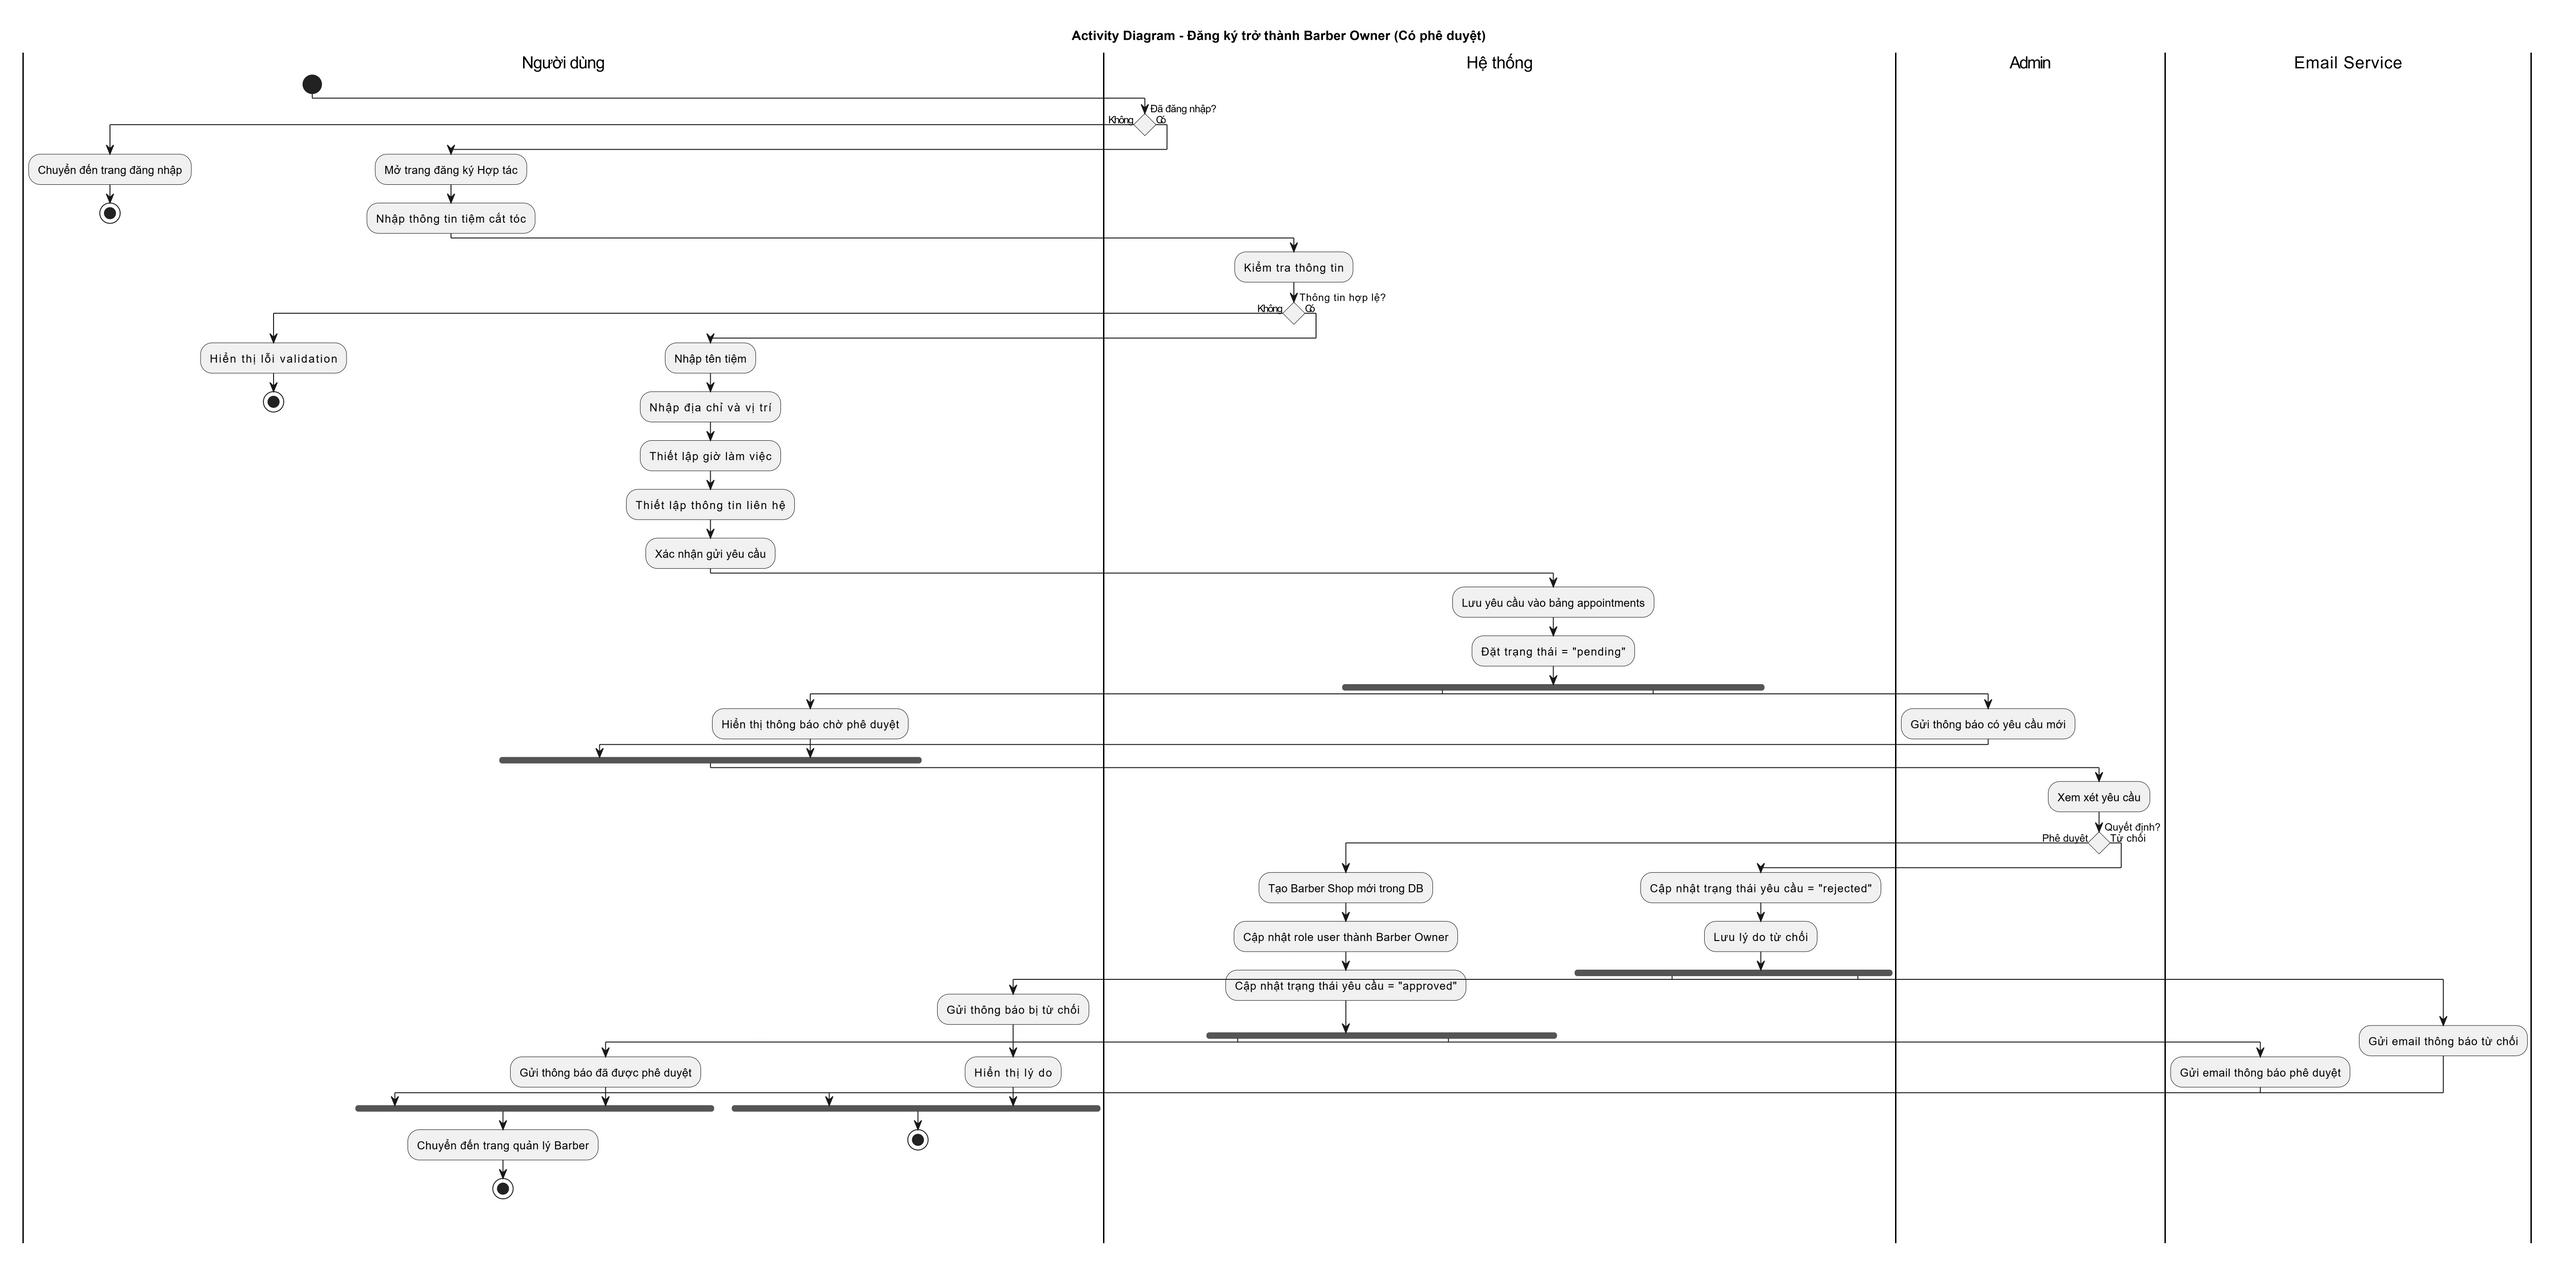
\includegraphics[width=0.8\textwidth]{figures/ac_hoptac_ok.jpg}
    \caption{Activity Diagram xử lý hợp tác}
    \label{fig:ac_hoptac}
\end{figure}


\textbf{Mục đích:} Cho phép người dùng đăng ký trở thành chủ tiệm cắt tóc thông qua quy trình xét duyệt từ Admin, bao gồm xác thực thông tin và phê duyệt hồ sơ.

\textbf{Luồng hoạt động:}

\begin{itemize}
    \item Hệ thống kiểm tra đăng nhập:
    \begin{itemize}
        \item \textit{Nếu chưa đăng nhập:} Chuyển đến trang đăng nhập và kết thúc.
        \item \textit{Nếu đã đăng nhập:} Mở trang đăng ký Hop tác.
    \end{itemize}
    \item Người dùng nhập thông tin hợp tác cắt tóc.
    \item Hệ thống kiểm tra thông tin đủ:
    \begin{itemize}
        \item \textit{Nếu không hợp đủ:} Hiển thị lỗi validation và kết thúc.
        \item \textit{Nếu đủ:} Nhập ảnh tiện.
    \end{itemize}
    \item Người dùng:
    \begin{itemize}
        \item Nhập ảnh chi vị trí
        \item Thiết lập giờ làm việc
        \item Thiết lập thông tin tiện hệ
        \item Xác nhận gửi yêu cầu
    \end{itemize}
    \item Hiển thị thông báo chờ phê duyệt.
    \item Admin:
    \begin{itemize}
        \item Lưu yêu cầu vào bảng appointments
        \item Đặt trạng thái = "pending"
    \end{itemize}
    \item Email Service gửi thông báo có yêu cầu mới.
    \item Admin xem sét yêu cầu và kiểm tra xét duyệt:
    \begin{itemize}
        \item \textit{Nếu từ chối:}
        \begin{itemize}
            \item Cập nhật trạng thái yêu cầu = "rejected"
            \item Lưu ý so từ chối
            \item Email Service gửi email thông báo từ chối
            \item Gửi email thông báo từ chối
            \item Gửi thông báo từ chối
            \item Hiển thị lý đủ
        \end{itemize}
        \item \textit{Nếu chấp nhận:}
        \begin{itemize}
            \item Tạo Barber Shop mới trong DB
            \item Cập nhật role user thành Barber Owner
            \item Cập nhật trạng thái yêu cầu = "approved"
            \item Gửi thông báo hô sở hợ phỉ duyệt
            \item Email Service gửi email thông báo phê duyệt
            \item Gửi email thông báo phê duyệt
        \end{itemize}
    \end{itemize}
    \item Gửi thông báo cho người phỉ duyệt.
    \item Chuyển đến trang quản lý Barber.
    \item Kết thúc quy trình.
\end{itemize}


\subsection{Activity Diagram cập nhật thông tin cá nhân người dùng}
\begin{figure}[H]
    \centering
    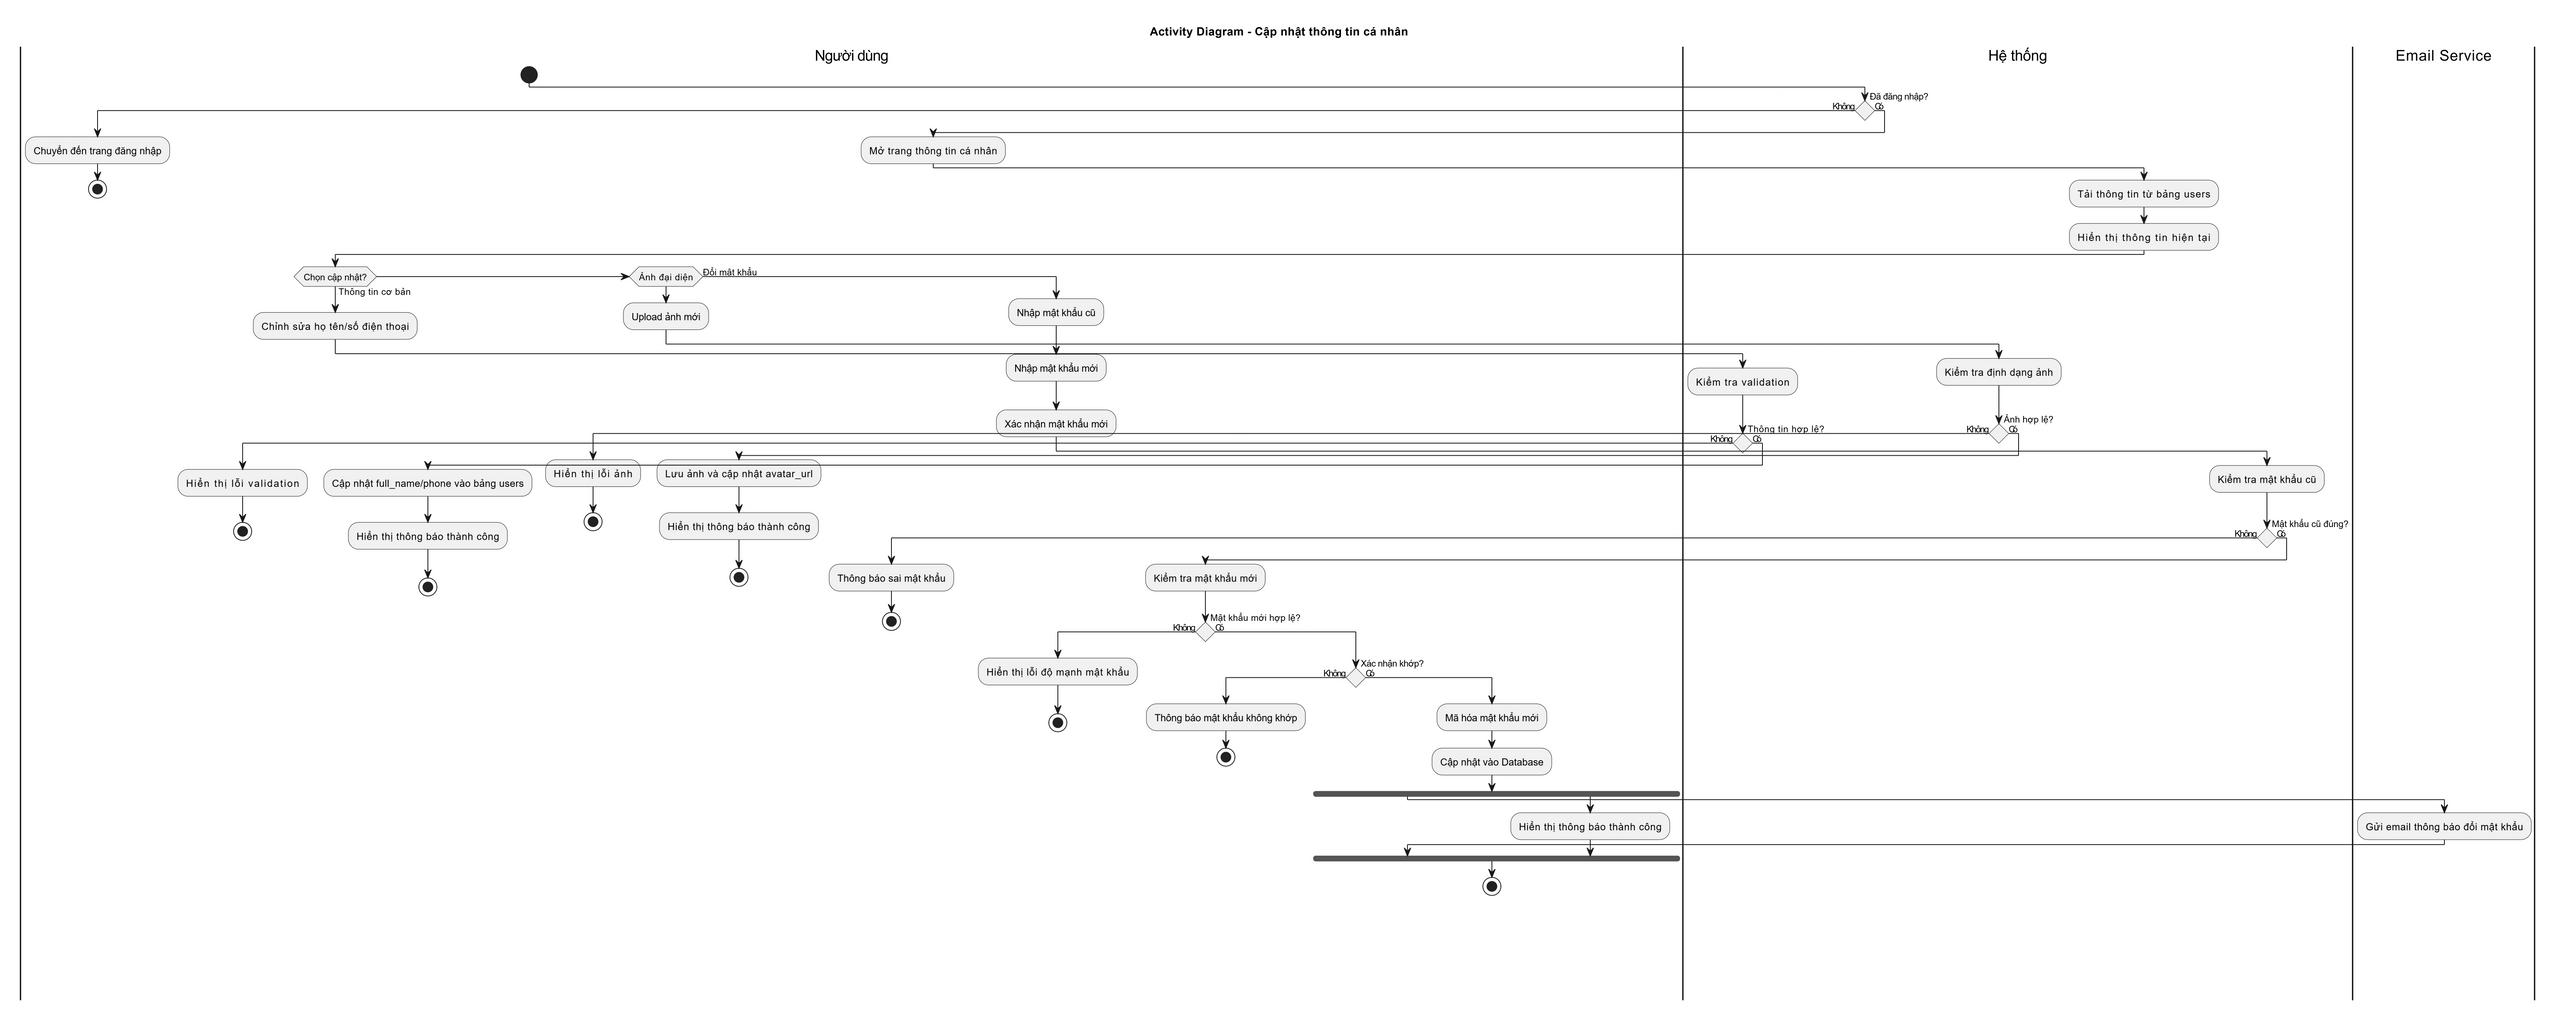
\includegraphics[width=0.8\textwidth]{figures/ac_update_profile.jpg}
    \caption{Activity Diagram cập nhật thông tin cá nhân}
    \label{fig:ac_update_profile}
\end{figure}


\textbf{Mục đích:} Cho phép người dùng cập nhật thông tin cá nhân bao gồm thông tin cơ bản, ảnh đại diện và đổi mật khẩu.

\textbf{Luồng hoạt động:}

\begin{itemize}
    \item Hệ thống kiểm tra đăng nhập:
    \begin{itemize}
        \item \textit{Nếu chưa đăng nhập:} Chuyển đến trang đăng nhập và kết thúc.
        \item \textit{Nếu đã đăng nhập:} Mở trang thông tin cá nhân.
    \end{itemize}
    \item Hệ thống tải thông tin từ bảng users và hiển thị thông tin hiện tại.
    \item Người dùng chọn loại cập nhật:
    
    \textbf{a) Thông tin cơ bản:}
    \begin{itemize}
        \item Chỉnh sửa họ tên/số điện thoại
        \item Hệ thống kiểm tra validation
        \item \textit{Nếu không hợp lệ:} Hiển thị lỗi validation và kết thúc
        \item \textit{Nếu hợp lệ:} Cập nhật full\_name/phone vào bảng users, hiển thị thông báo thành công
    \end{itemize}
    
    \textbf{b) Ảnh đại diện:}
    \begin{itemize}
        \item Upload ảnh mới
        \item Hệ thống kiểm tra định dạng ảnh
        \item \textit{Nếu không hợp lệ:} Hiển thị lỗi ảnh và kết thúc
        \item \textit{Nếu hợp lệ:} Lưu ảnh và cập nhật avatar\_url, hiển thị thông báo thành công
    \end{itemize}
    
    \textbf{c) Đổi mật khẩu:}
    \begin{itemize}
        \item Nhập mật khẩu cũ, mật khẩu mới và xác nhận mật khẩu mới
        \item Kiểm tra mật khẩu cũ đúng:
        \begin{itemize}
            \item \textit{Nếu sai:} Thông báo sai mật khẩu và kết thúc
            \item \textit{Nếu đúng:} Kiểm tra mật khẩu mới hợp lệ
        \end{itemize}
        \item Kiểm tra độ mạnh mật khẩu mới:
        \begin{itemize}
            \item \textit{Nếu không hợp lệ:} Hiển thị lỗi độ mạnh mật khẩu và kết thúc
            \item \textit{Nếu hợp lệ:} Kiểm tra xác nhận khớp
        \end{itemize}
        \item Kiểm tra xác nhận mật khẩu:
        \begin{itemize}
            \item \textit{Nếu không khớp:} Thông báo mật khẩu không khớp và kết thúc
            \item \textit{Nếu khớp:} Mã hóa mật khẩu mới, cập nhật vào database
        \end{itemize}
        \item Thực hiện song song:
        \begin{itemize}
            \item Email Service gửi email thông báo đổi mật khẩu
            \item Hiển thị thông báo thành công
        \end{itemize}
    \end{itemize}
\end{itemize}


\subsection{Activity Diagram tra cứu tiệm cắt tóc}
\begin{figure}[H]
    \centering
    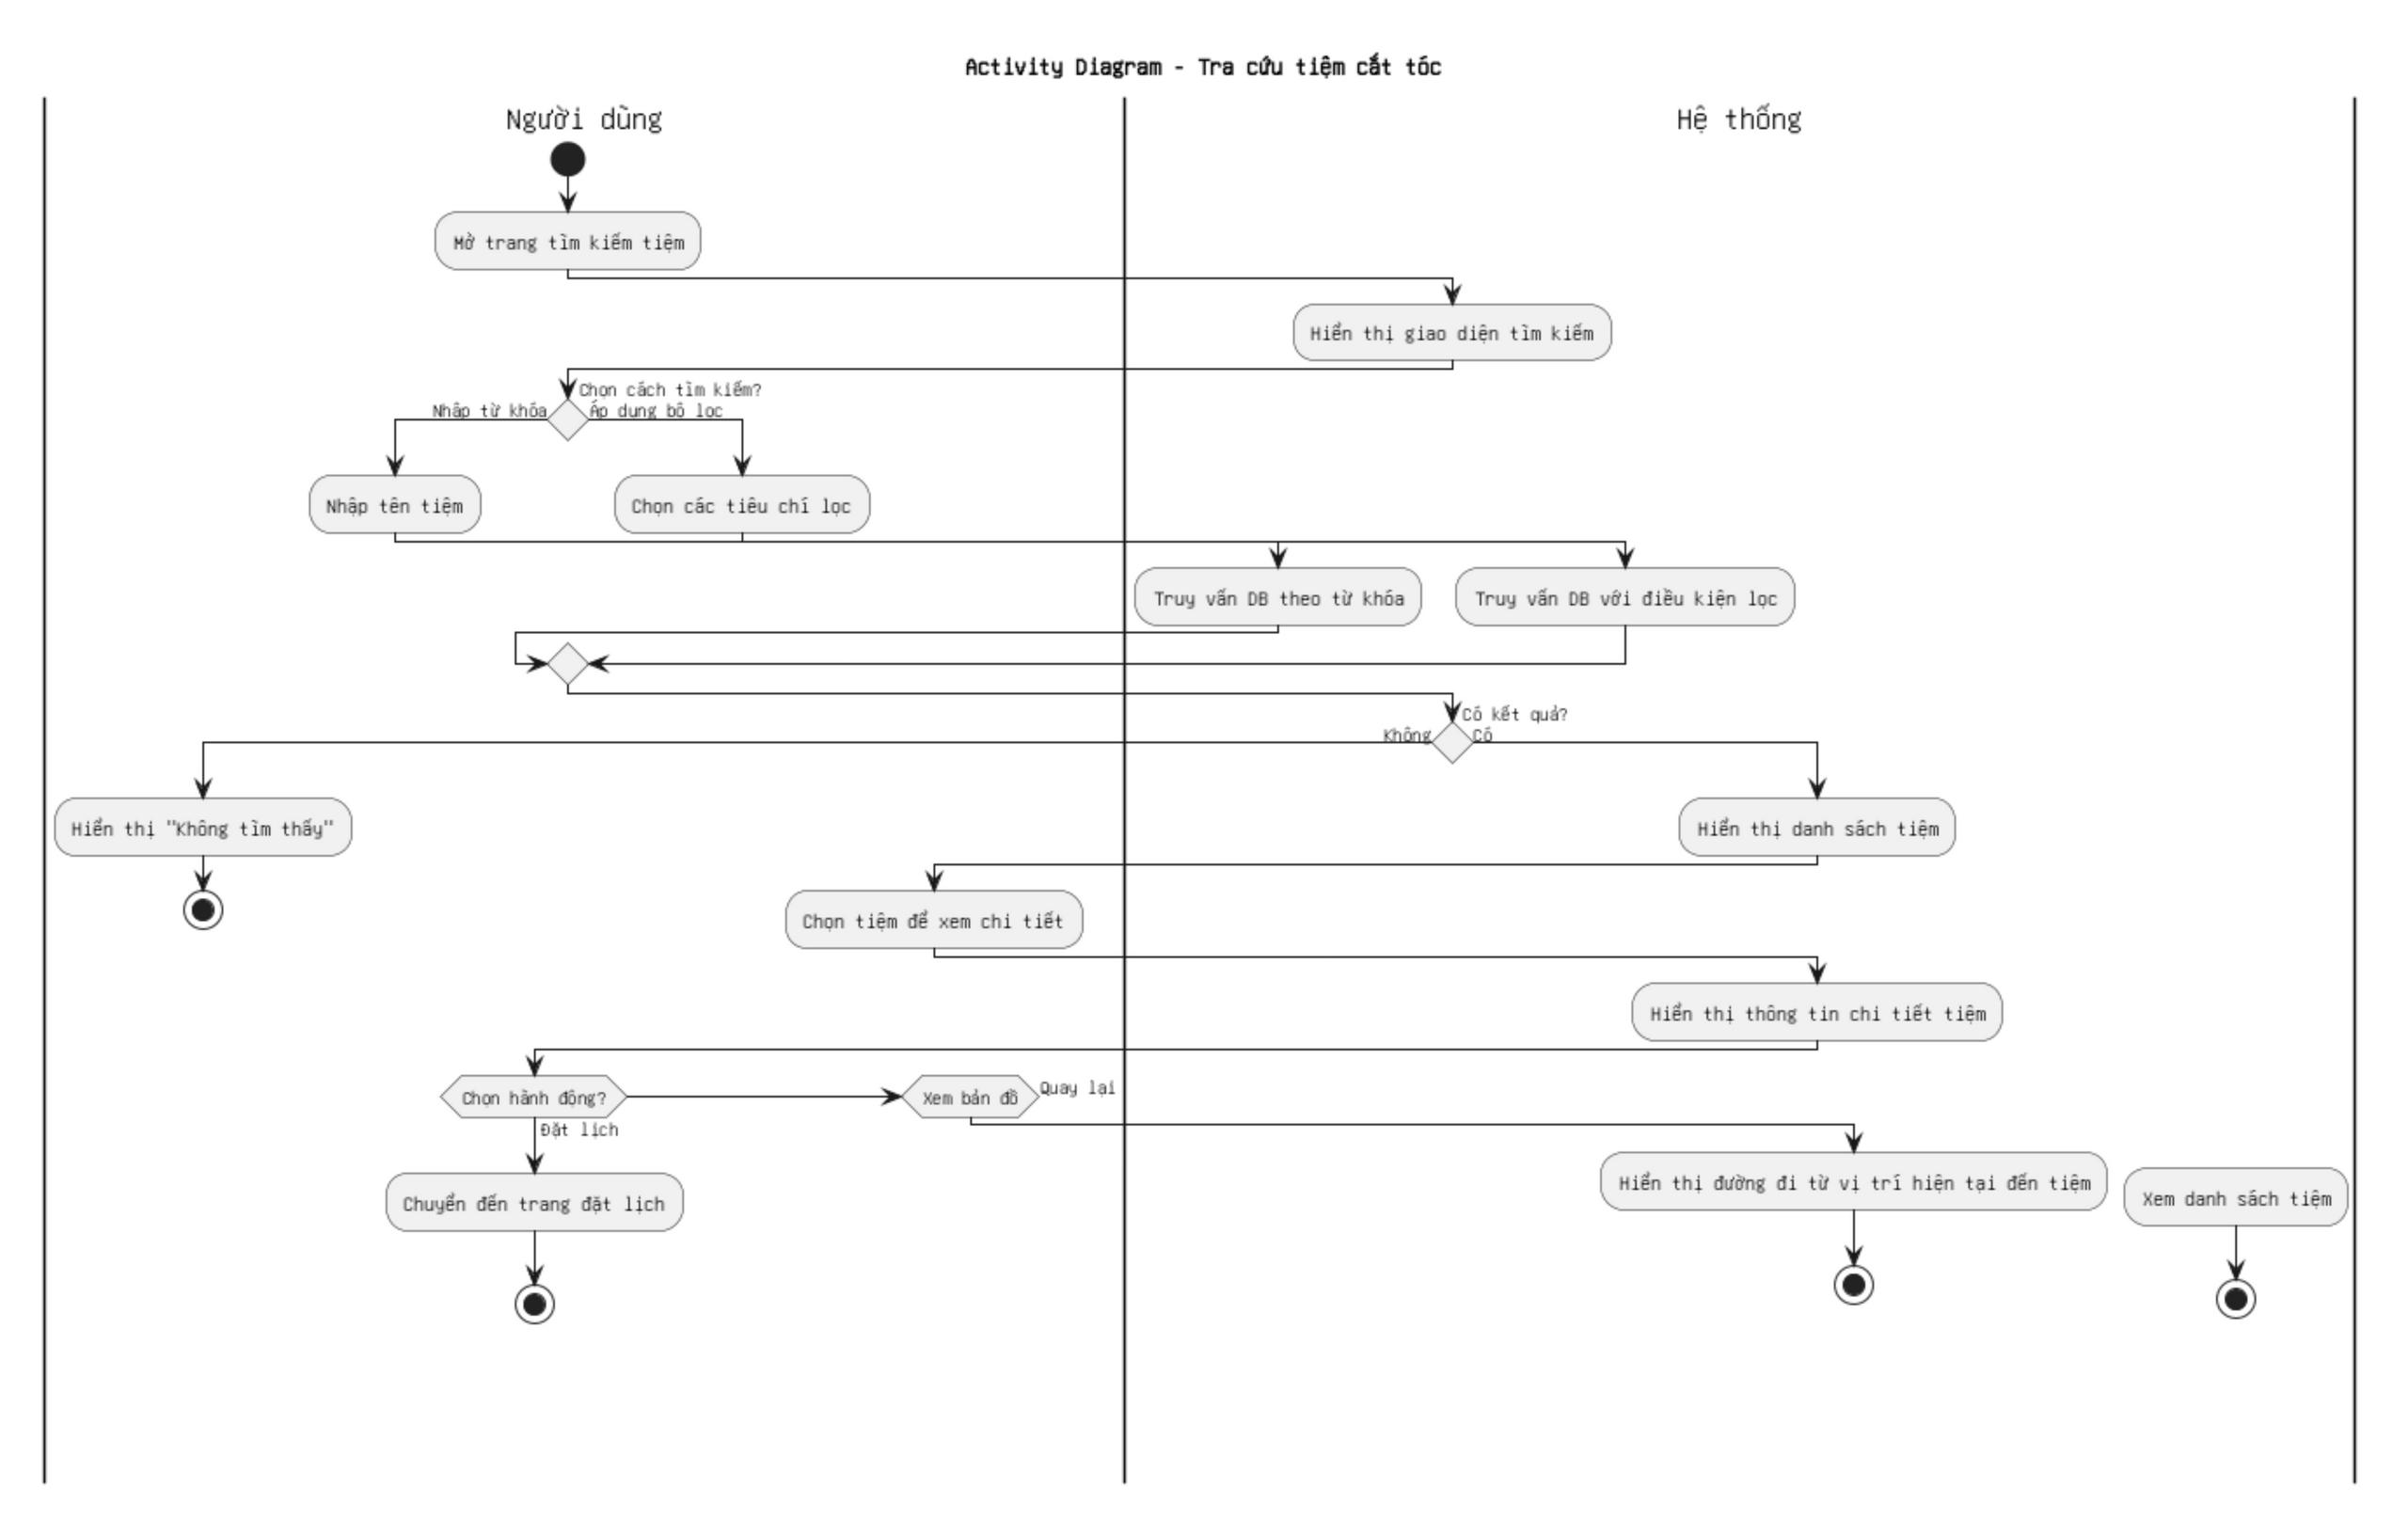
\includegraphics[width=1\textwidth]{figures/ac_tra_cuu.jpg}
    \caption{Activity Diagram tra cứu tiệm cắt tóc}
    \label{fig:ac_tra_cuu}
\end{figure}
\textbf{Mục đích:} Cho phép người dùng tìm kiếm và tra cứu thông tin các tiệm cắt tóc theo tên hoặc theo các tiêu chí lọc.

\textbf{Luồng hoạt động:}

\begin{itemize}
    \item Người dùng mở trang tìm kiếm tiệm.
    \item Hệ thống hiển thị giao diện tìm tiệm.
    \item Người dùng chọn cách tìm kiếm:
    
    \textbf{a) Nhập từ khóa:}
    \begin{itemize}
        \item Nhập tên tiệm
        \item Hệ thống truy vấn DB theo từ khóa
    \end{itemize}
    
    \textbf{b) Chọn các tiêu chí lọc:}
    \begin{itemize}
        \item Chọn các tiêu chí lọc
        \item Hệ thống truy vấn DB với điều kiện lọc
    \end{itemize}
    
    \item Hệ thống kiểm tra có kết quả:
    \begin{itemize}
        \item \textit{Nếu không:} Hiển thị "Không tìm thấy" và kết thúc.
        \item \textit{Nếu có:} Hiển thị danh sách tiệm.
    \end{itemize}
    
    \item Người dùng chọn tiệm để xem chi tiết.
    \item Hệ thống hiển thị thông tin chi tiết tiệm.
    \item Người dùng chọn hành động:
    \begin{itemize}
        \item \textit{Đặt lịch:} Chuyển đến trang đặt lịch và kết thúc.
        \item \textit{Quay lại:} Xem danh sách tiệm và kết thúc.
    \end{itemize}
    
    \item Hiển thị đường đi từ vị trí hiện tại đến tiệm và kết thúc.
\end{itemize}

\subsection{Activity Diagram cập nhật thông tin tiệm cắt tóc}
\begin{figure}[H]
    \centering
    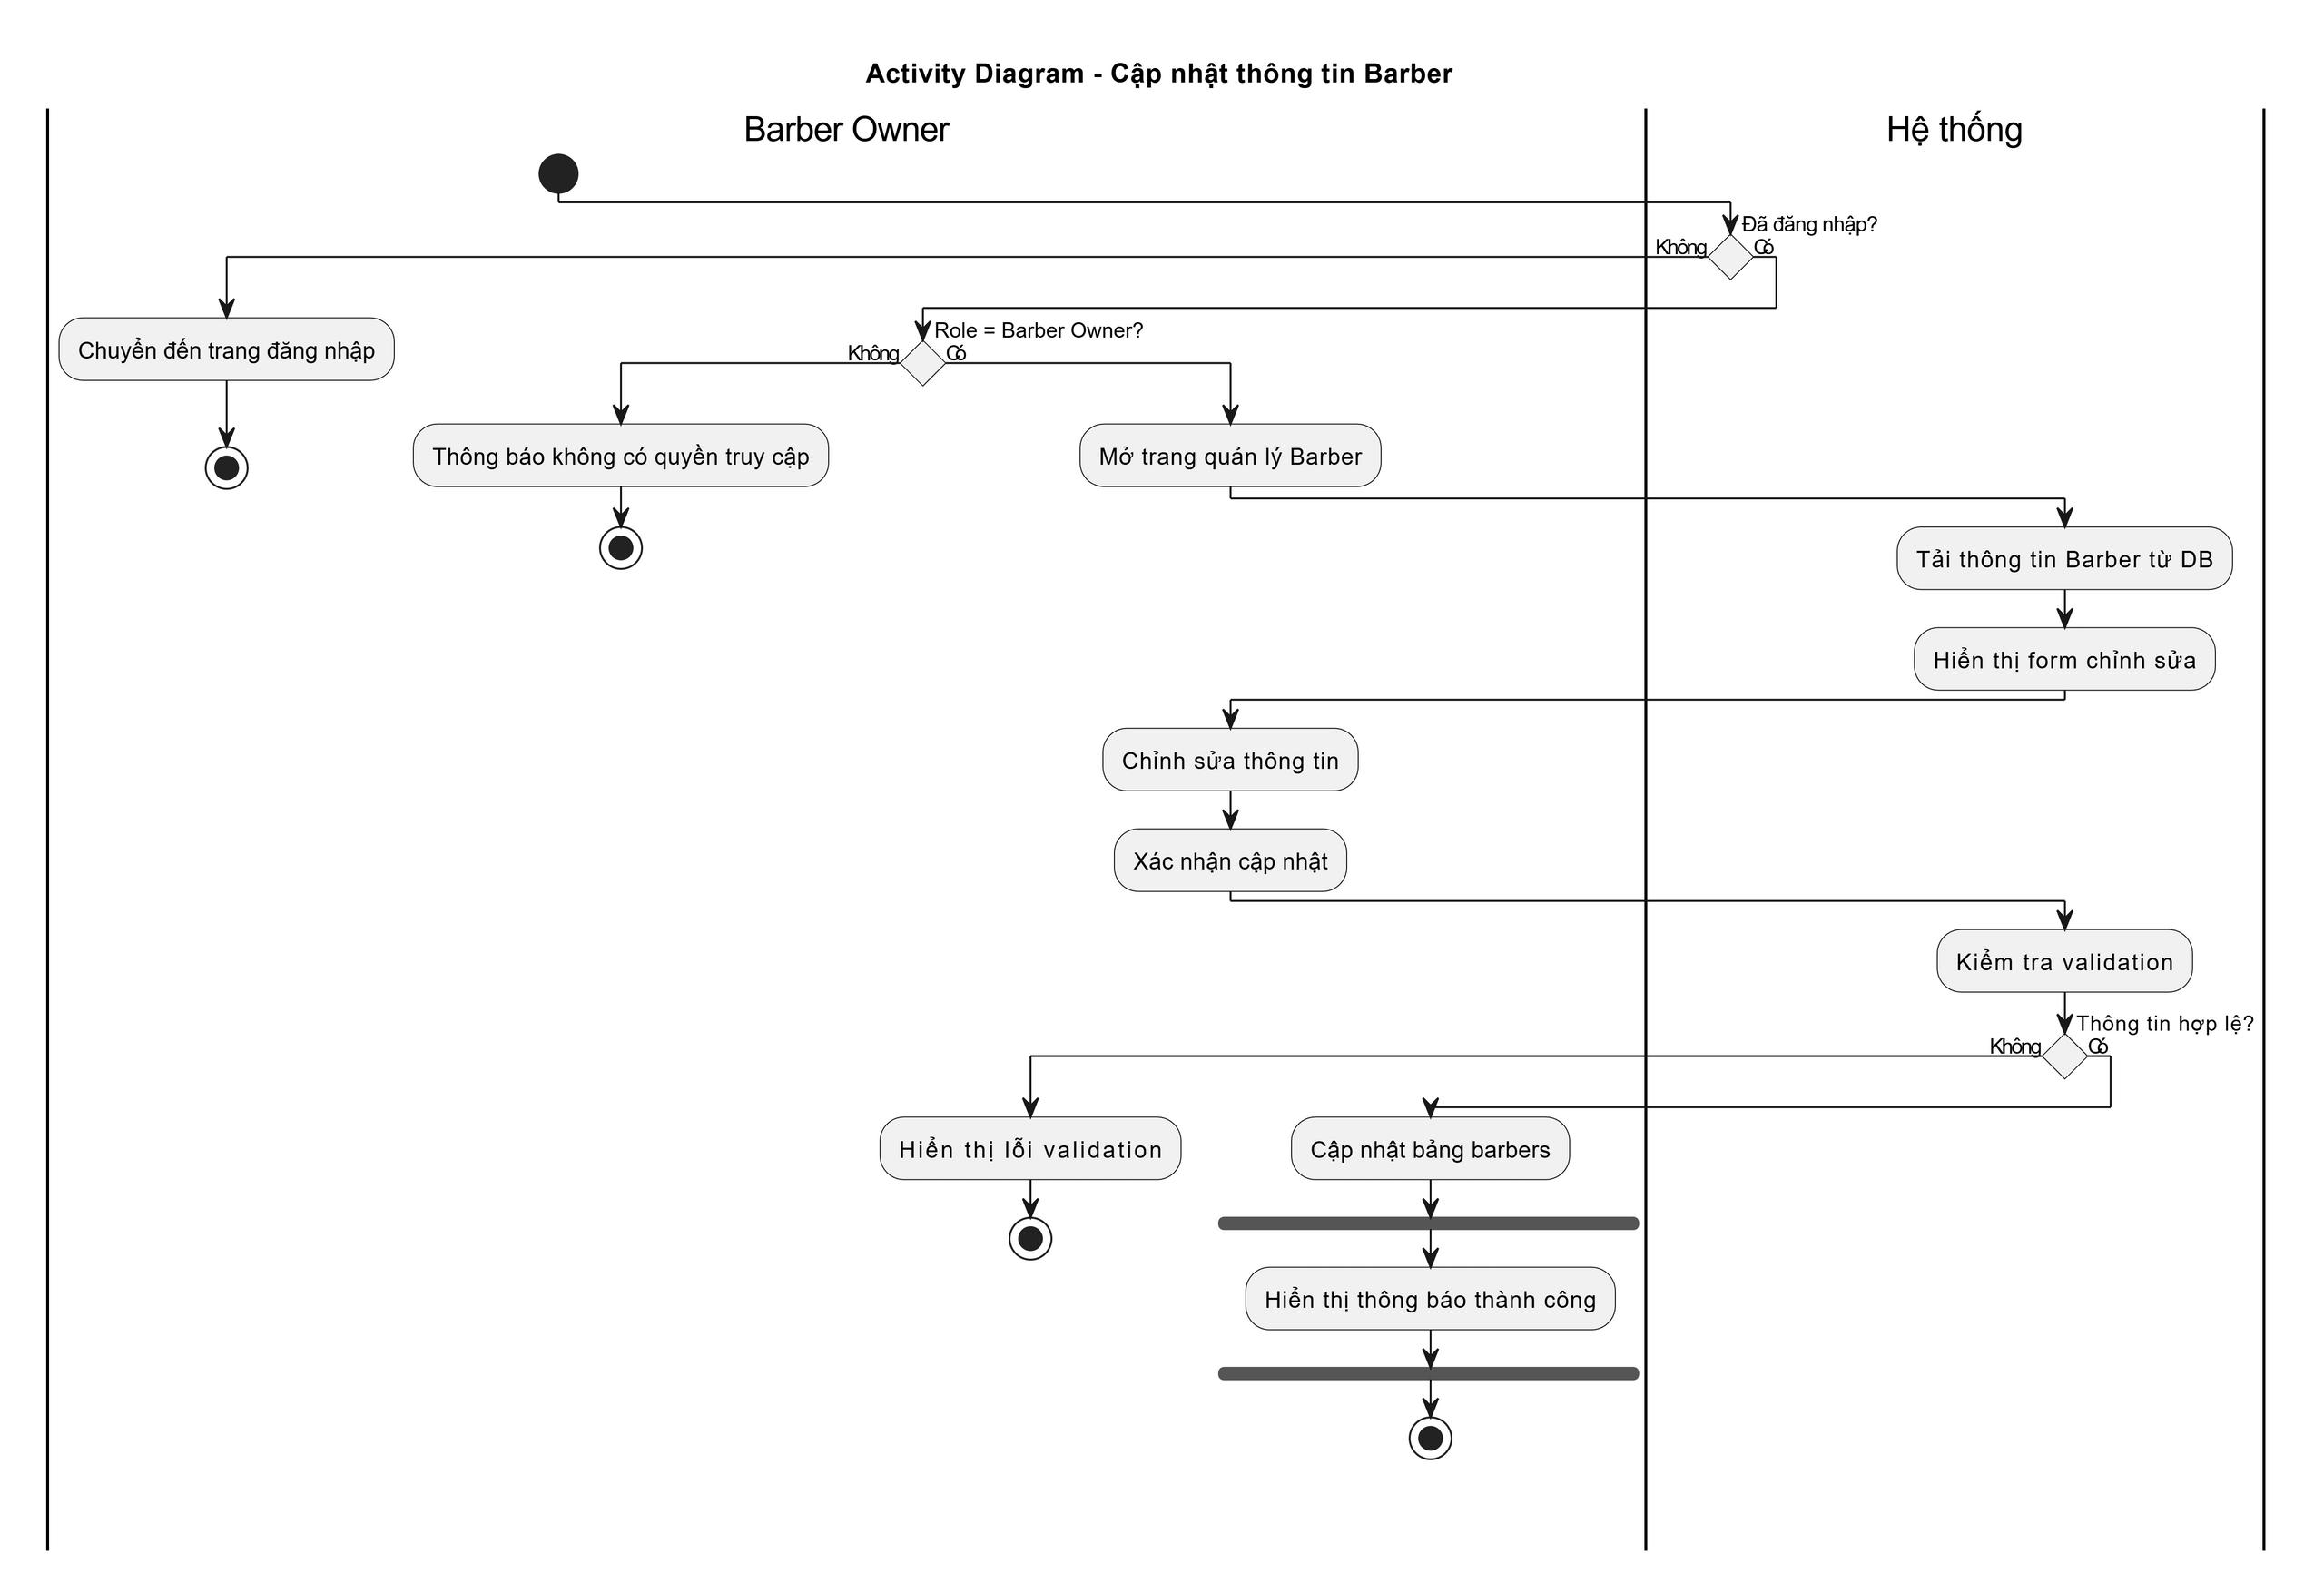
\includegraphics[width=1.2\textwidth]{figures/ac_update_ower.jpg}
    \caption{Activity Diagram cập nhật thông tin tiệm cắt tóc}
    \label{fig:ac_update_ower}
\end{figure}


\textbf{Mục đích:} Cho phép Barber Owner chỉnh sửa và cập nhật thông tin tiệm cắt tóc của mình trong hệ thống.

\textbf{Luồng hoạt động:}

\begin{itemize}
    \item Hệ thống kiểm tra đăng nhập:
    \begin{itemize}
        \item \textit{Nếu chưa đăng nhập:} Chuyển đến trang đăng nhập và kết thúc.
        \item \textit{Nếu đã đăng nhập:} Kiểm tra quyền truy cập.
    \end{itemize}
    
    \item Hệ thống kiểm tra Role = Barber Owner:
    \begin{itemize}
        \item \textit{Nếu không:} Thông báo không có quyền truy cập và kết thúc.
        \item \textit{Nếu có:} Mở trang quản lý Barber.
    \end{itemize}
    
    \item Hệ thống tải thông tin Barber từ DB và hiển thị form chỉnh sửa.
    
    \item Barber Owner chỉnh sửa thông tin.
    
    \item Barber Owner xác nhận cập nhật.
    
    \item Hệ thống kiểm tra validation:
    \begin{itemize}
        \item \textit{Nếu không hợp lệ:} Hiển thị lỗi validation và kết thúc.
        \item \textit{Nếu hợp lệ:} Cập nhật bảng barbers.
    \end{itemize}
    
    \item Hiển thị thông báo thành công.
    
    \item Kết thúc quy trình.
\end{itemize}

\subsection{Activity Diagram xem tài liệu RAG}
\begin{figure}[H]
    \centering
    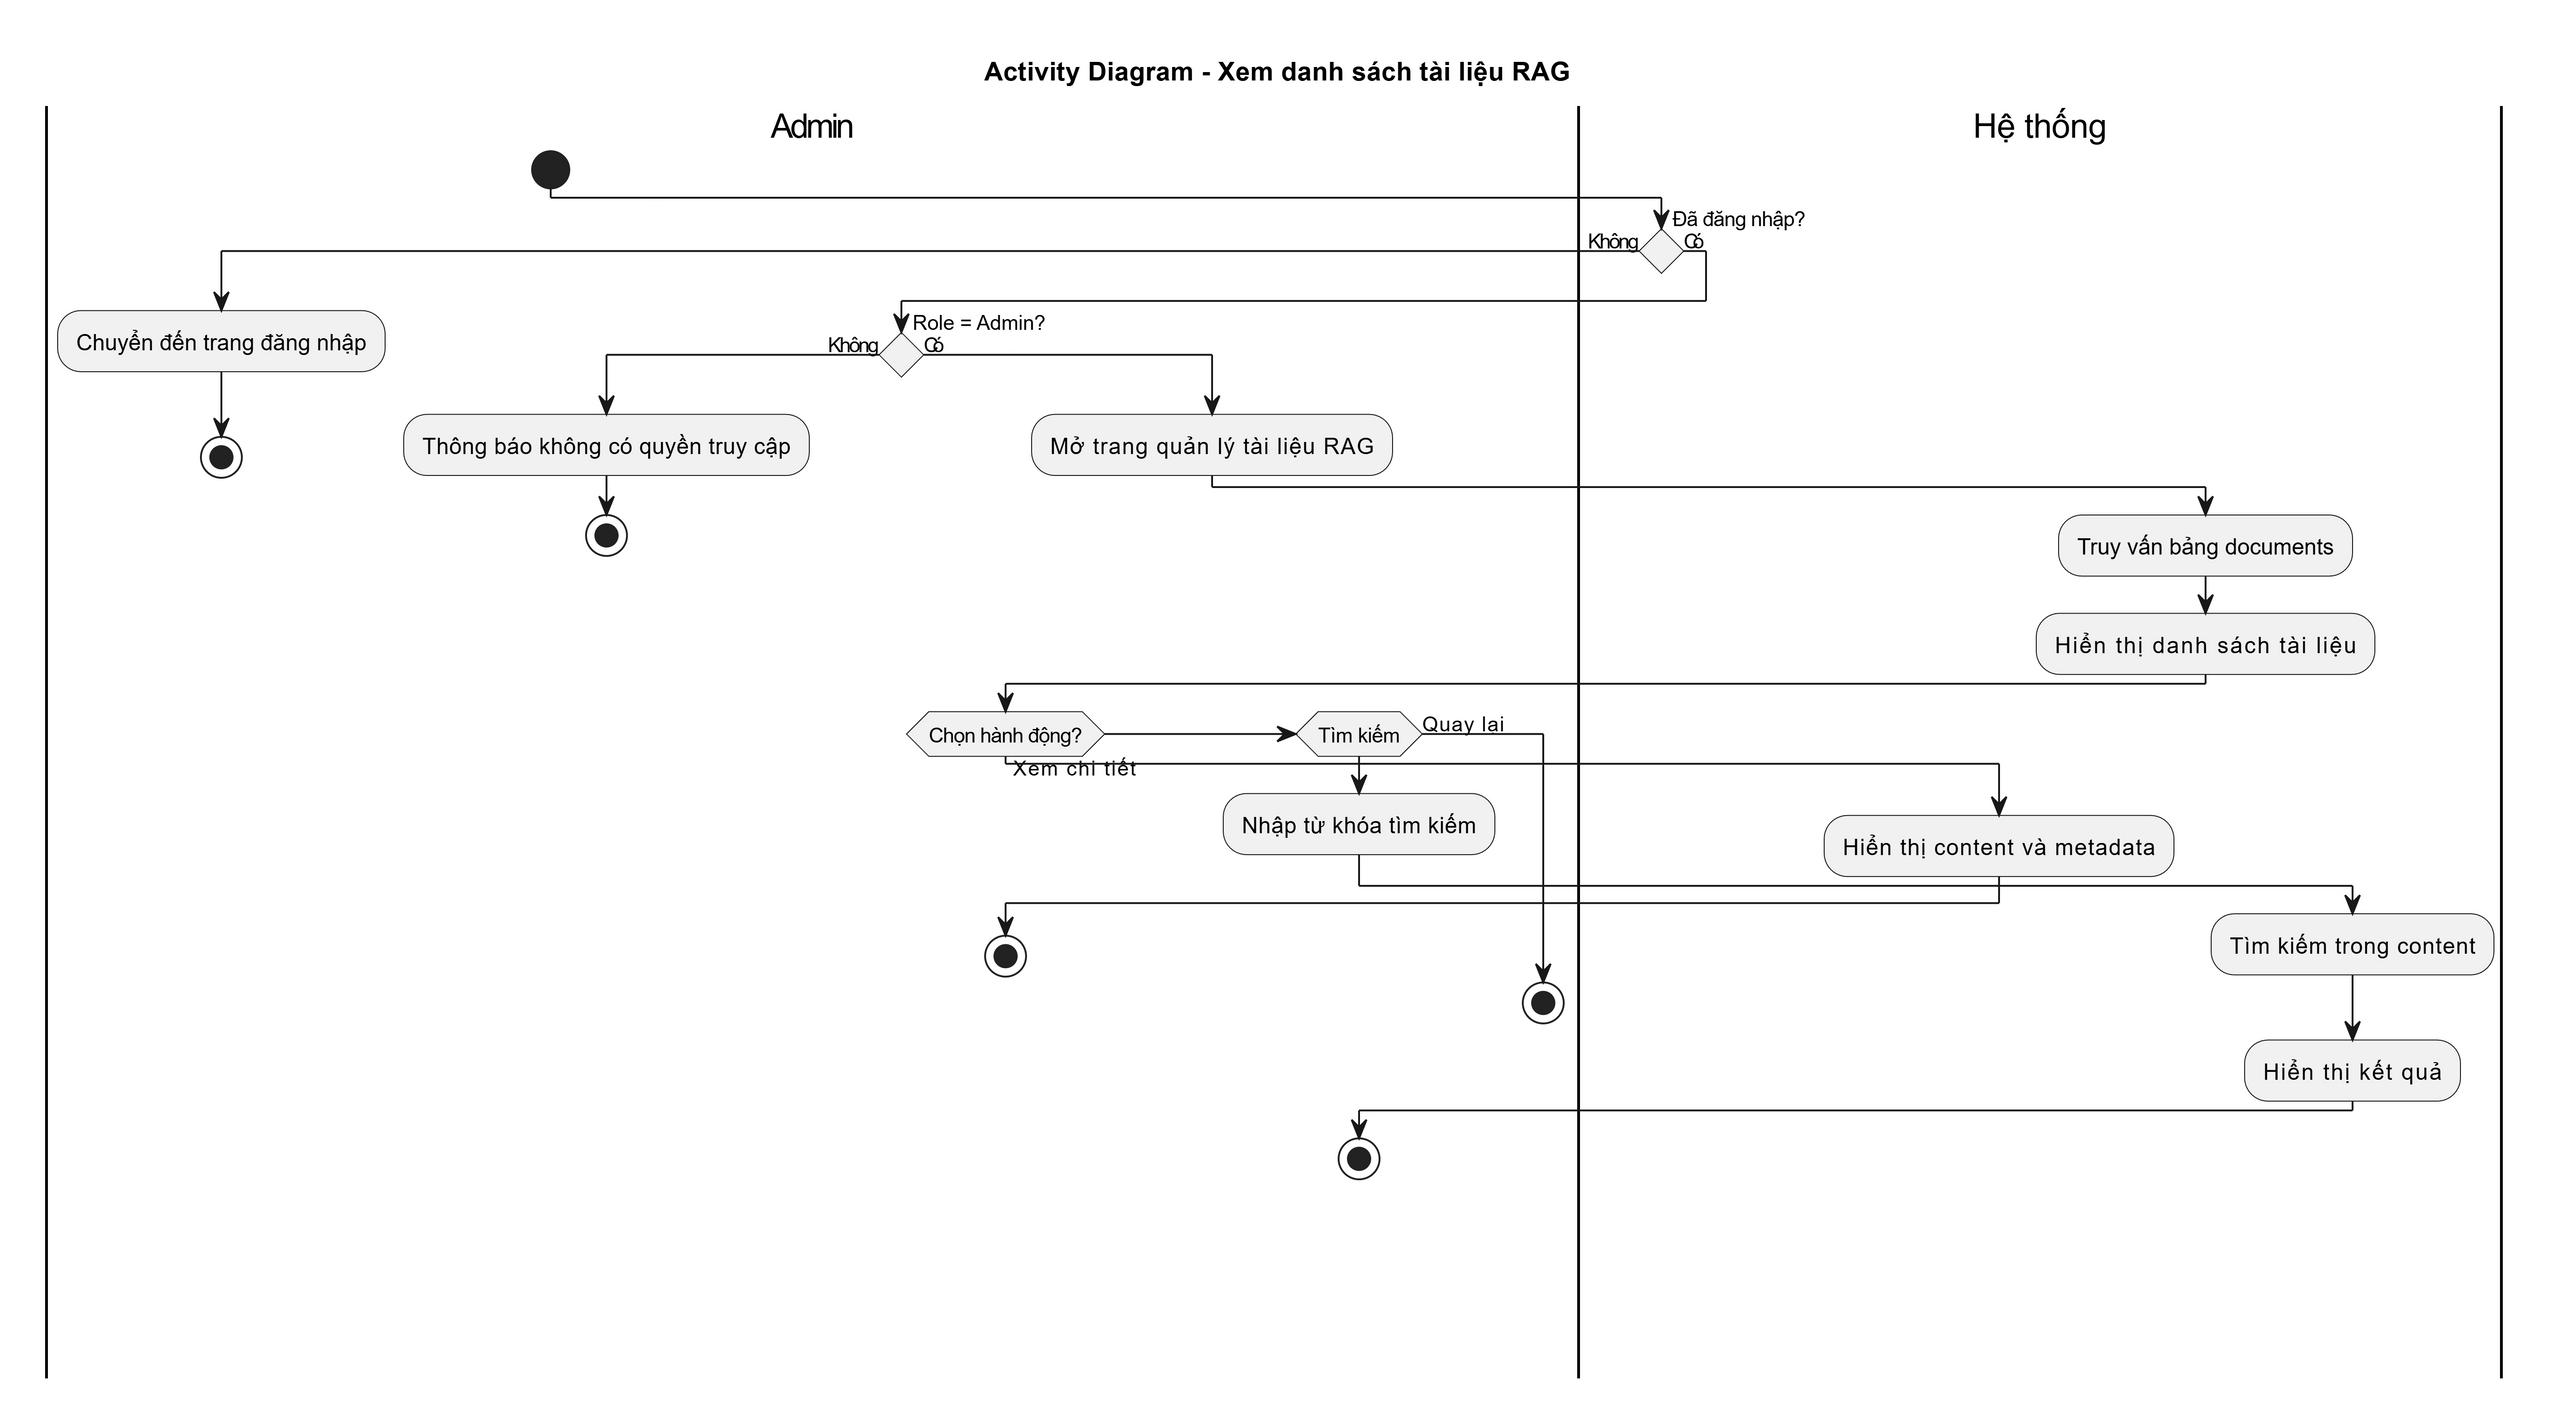
\includegraphics[width=0.8\textwidth]{figures/ac_rag.jpg}
    \caption{Activity Diagram xem tài liệu RAG}
    \label{fig:xem_rag}
\end{figure}

\textbf{Mục đích:} Cho phép Admin xem và quản lý danh sách tài liệu trong hệ thống RAG (Retrieval-Augmented Generation) để phục vụ chatbot tư vấn.

\textbf{Luồng hoạt động:}

\begin{itemize}
    \item Hệ thống kiểm tra đăng nhập:
    \begin{itemize}
        \item \textit{Nếu chưa đăng nhập:} Chuyển đến trang đăng nhập và kết thúc.
        \item \textit{Nếu đã đăng nhập:} Kiểm tra quyền truy cập.
    \end{itemize}
    
    \item Hệ thống kiểm tra Role = Admin:
    \begin{itemize}
        \item \textit{Nếu không:} Thông báo không có quyền truy cập và kết thúc.
        \item \textit{Nếu có:} Mở trang quản lý tài liệu RAG.
    \end{itemize}
    
    \item Hệ thống truy vấn bảng documents và hiển thị danh sách tài liệu.
    
    \item Admin chọn hành động:
    \begin{itemize}
        \item \textit{Xem chi tiết:}
        \begin{itemize}
            \item Hiển thị content và metadata
            \item Tìm kiếm trong content
            \item Hiển thị kết quả
            \item Kết thúc
        \end{itemize}
        \item \textit{Tìm kiếm:}
        \begin{itemize}
            \item Nhập từ khóa tìm kiếm
            \item Kết thúc
        \end{itemize}
        \item \textit{Quay lại:} Kết thúc
    \end{itemize}
\end{itemize}

\subsection{Activity Diagram tạo vector database}
\begin{figure}[H]
    \centering
    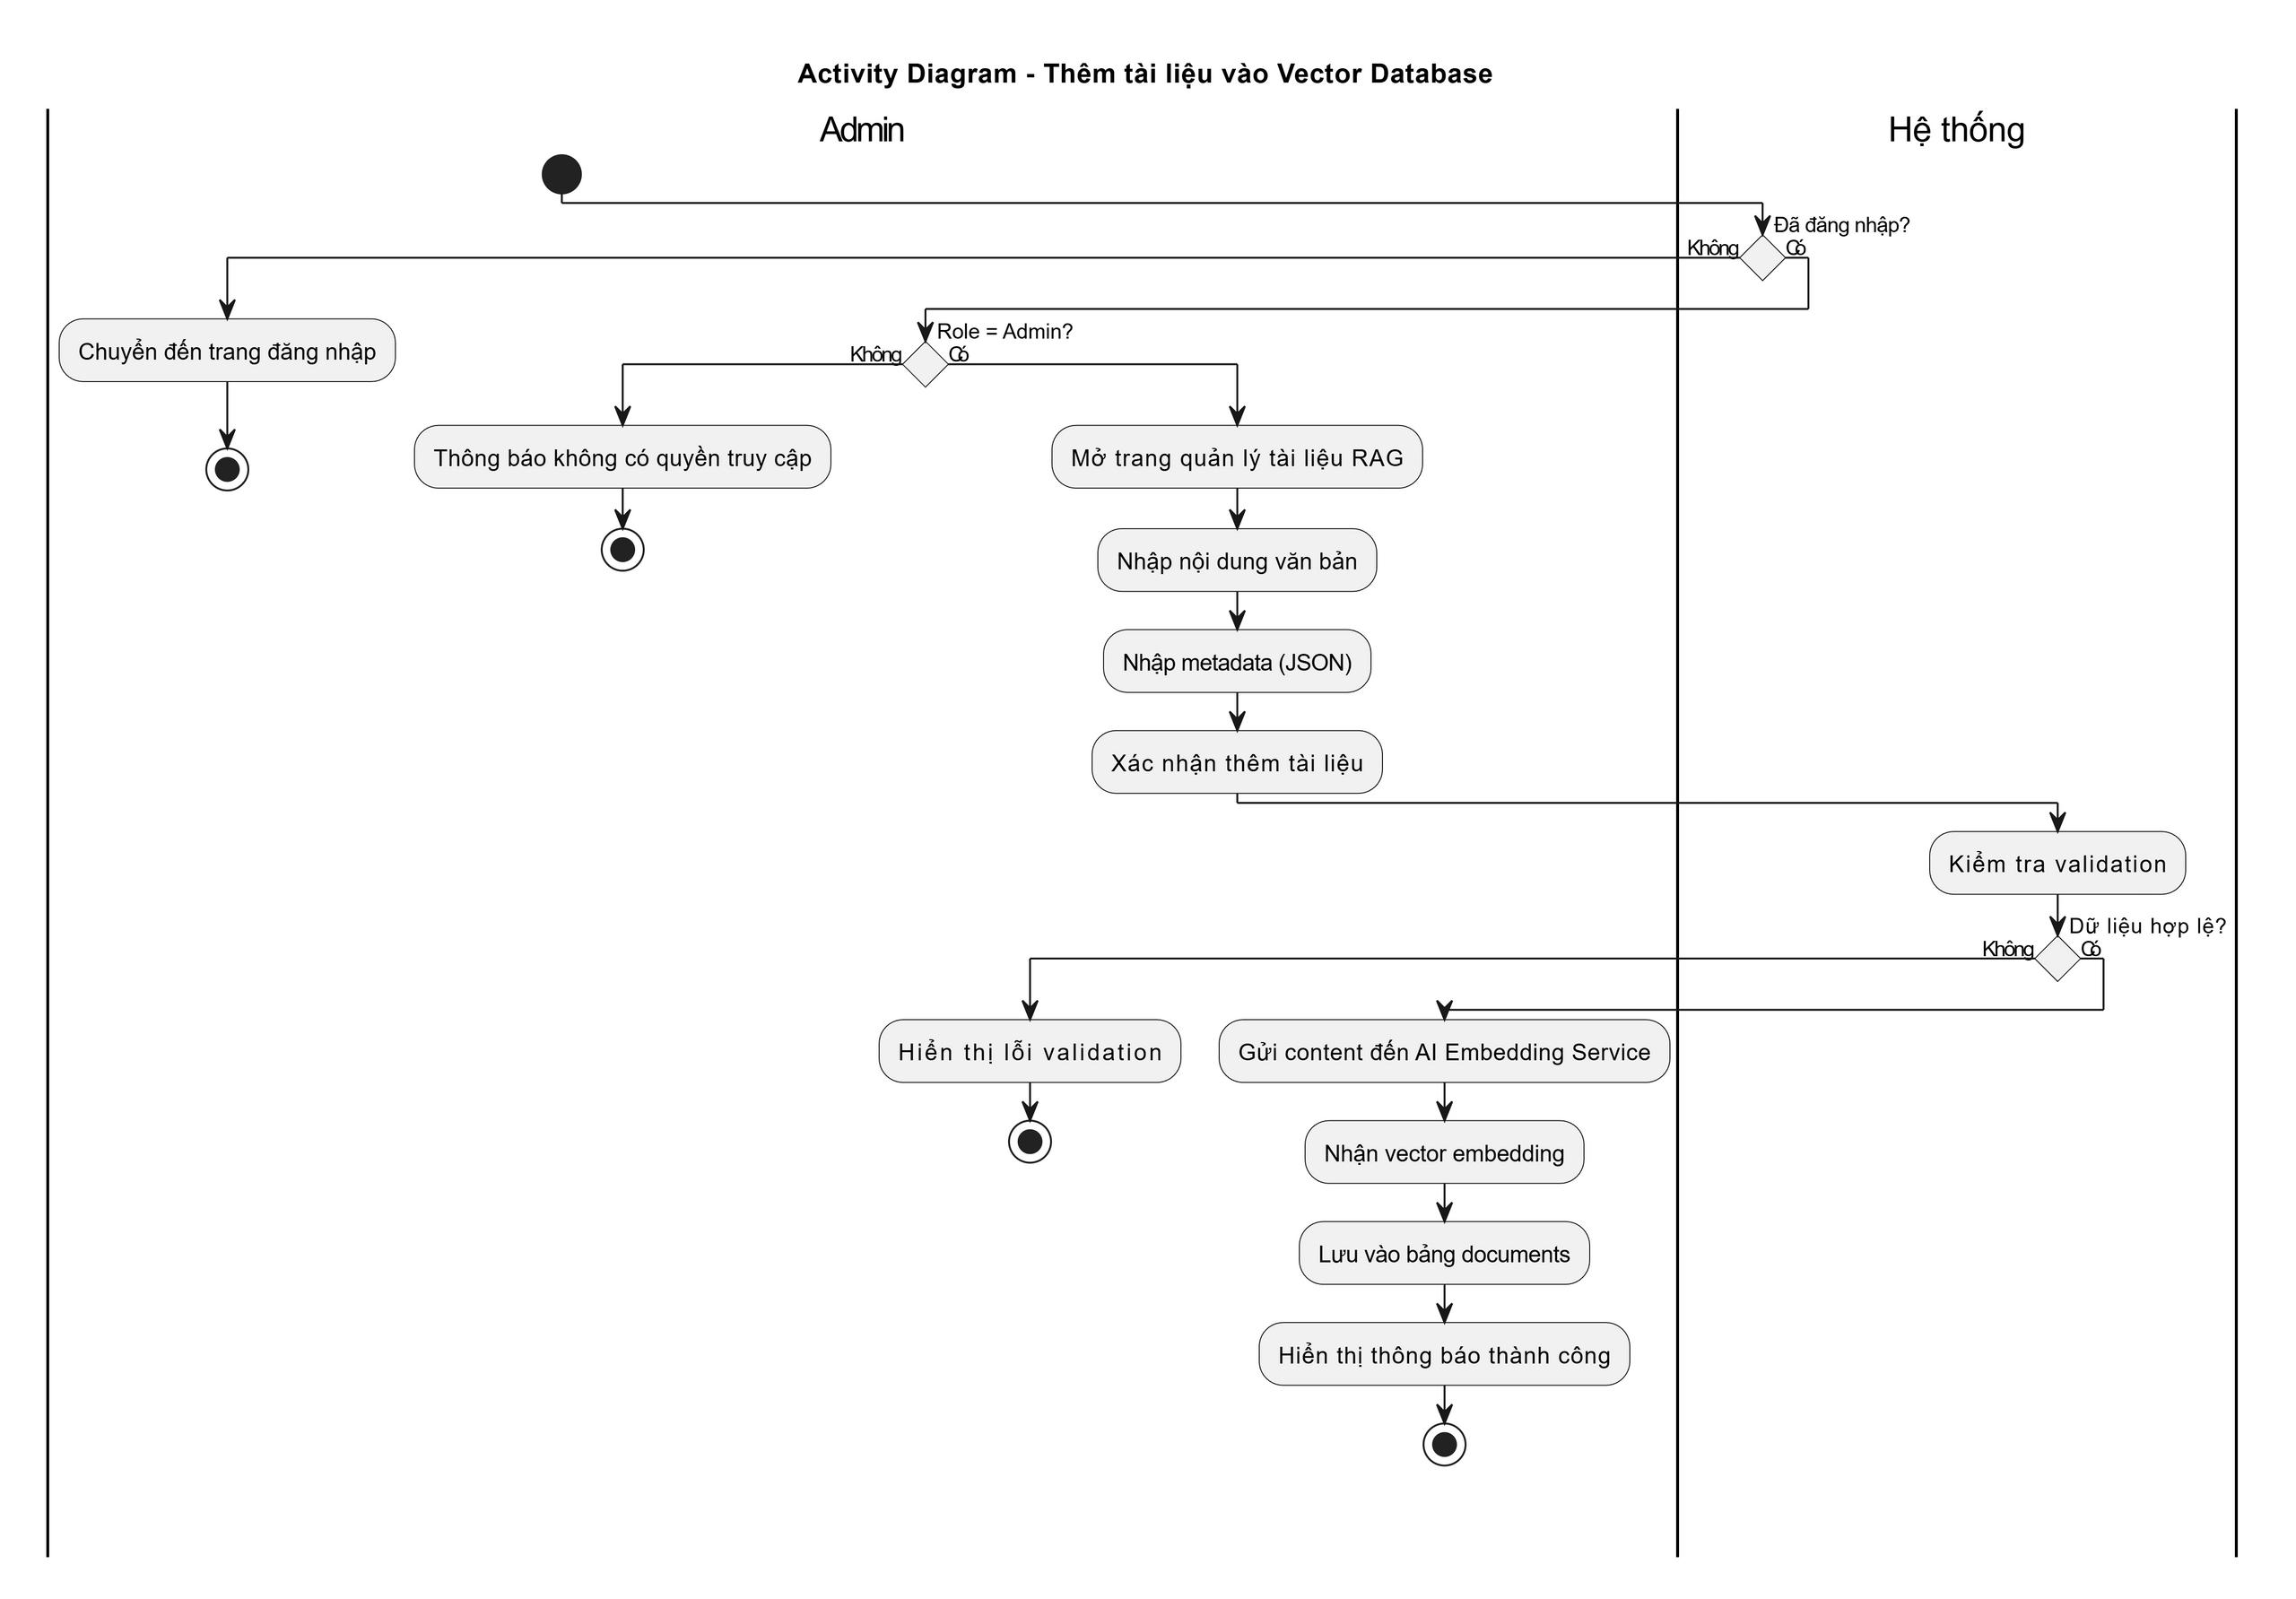
\includegraphics[width=0.8\textwidth]{figures/ac_vecto_database.jpg}
    \caption{Activity Diagram tạo vector database}
    \label{fig:ac_vector_db}
\end{figure}

\textbf{Mục đích:} Cho phép Admin thêm tài liệu mới vào Vector Database để tăng cường khả năng tư vấn của chatbot RAG.

\textbf{Luồng hoạt động:}

\begin{itemize}
    \item Hệ thống kiểm tra đăng nhập:
    \begin{itemize}
        \item \textit{Nếu chưa đăng nhập:} Chuyển đến trang đăng nhập và kết thúc.
        \item \textit{Nếu đã đăng nhập:} Kiểm tra quyền truy cập.
    \end{itemize}
    
    \item Hệ thống kiểm tra Role = Admin:
    \begin{itemize}
        \item \textit{Nếu không:} Thông báo không có quyền truy cập và kết thúc.
        \item \textit{Nếu có:} Mở trang quản lý tài liệu RAG.
    \end{itemize}
    
    \item Admin nhập nội dung văn bản.
    
    \item Admin nhập metadata (JSON).
    
    \item Admin xác nhận thêm tài liệu.
    
    \item Hệ thống kiểm tra validation:
    \begin{itemize}
        \item \textit{Nếu không hợp lệ:} Hiển thị lỗi validation và kết thúc.
        \item \textit{Nếu hợp lệ:} Gửi content đến AI Embedding Service.
    \end{itemize}
    
    \item Nhận vector embedding từ AI service.
    
    \item Lưu vào bảng documents.
    
    \item Hiển thị thông báo thành công.
    
    \item Kết thúc quy trình.
\end{itemize}

\subsection{Activity Diagram cập nhật tài liệu RAG}
\begin{figure}[H]
    \centering
    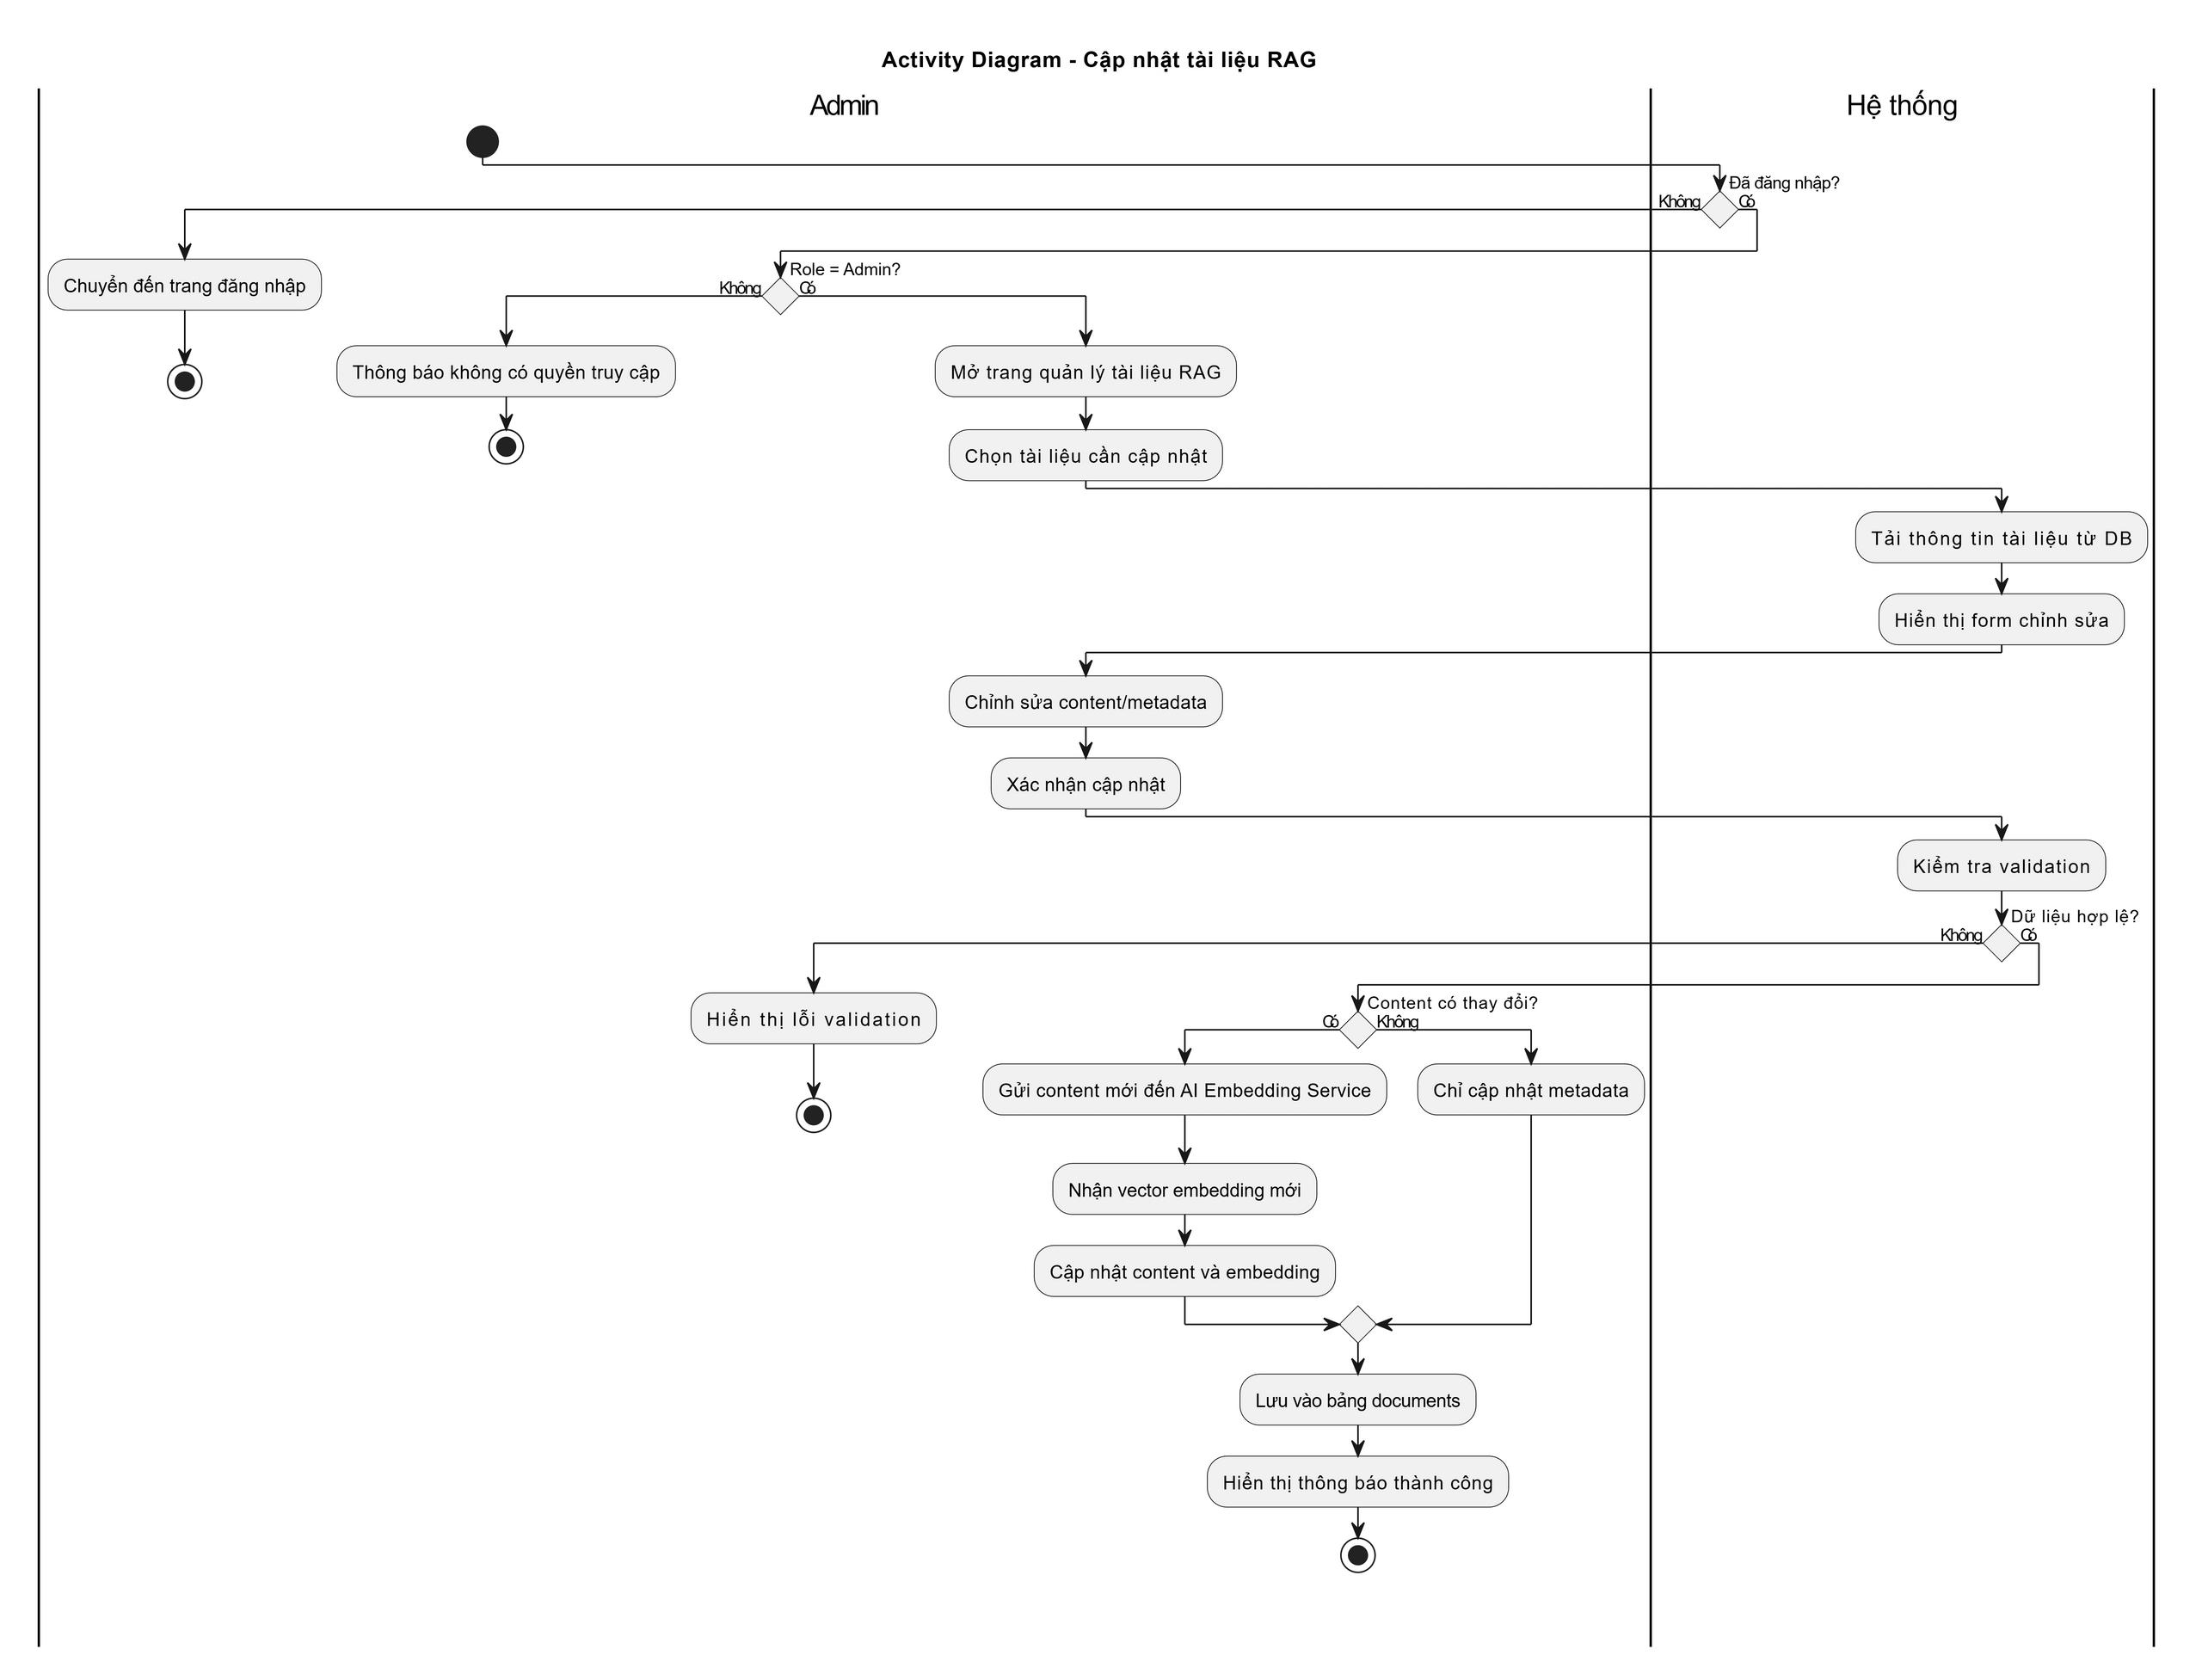
\includegraphics[width=0.8\textwidth]{figures/ac_update_rag.jpg}
    \caption{Activity Diagram cập nhật tài liệu RAG}
    \label{fig:ac_update_rag}
\end{figure}
\textbf{Mục đích:} Cho phép Admin chỉnh sửa và cập nhật thông tin tài liệu trong Vector Database để cải thiện chất lượng tư vấn của chatbot RAG.

\textbf{Luồng hoạt động:}

\begin{itemize}
    \item Hệ thống kiểm tra đăng nhập:
    \begin{itemize}
        \item \textit{Nếu chưa đăng nhập:} Chuyển đến trang đăng nhập và kết thúc.
        \item \textit{Nếu đã đăng nhập:} Kiểm tra quyền truy cập.
    \end{itemize}
    
    \item Hệ thống kiểm tra Role = Admin:
    \begin{itemize}
        \item \textit{Nếu không:} Thông báo không có quyền truy cập và kết thúc.
        \item \textit{Nếu có:} Mở trang quản lý tài liệu RAG.
    \end{itemize}
    
    \item Admin chọn tài liệu cần cập nhật.
    
    \item Hệ thống tải thông tin tài liệu từ DB và hiển thị form chỉnh sửa.
    
    \item Admin chỉnh sửa content/metadata.
    
    \item Admin xác nhận cập nhật.
    
    \item Hệ thống kiểm tra validation:
    \begin{itemize}
        \item \textit{Nếu không hợp lệ:} Hiển thị lỗi validation và kết thúc.
        \item \textit{Nếu hợp lệ:} Kiểm tra content có thay đổi.
    \end{itemize}
    
    \item Hệ thống kiểm tra content có thay đổi:
    \begin{itemize}
        \item \textit{Nếu có:}
        \begin{itemize}
            \item Gửi content mới đến AI Embedding Service
            \item Nhận vector embedding mới
            \item Cập nhật content và embedding
        \end{itemize}
        \item \textit{Nếu không:} Chỉ cập nhật metadata.
    \end{itemize}
    
    \item Lưu vào bảng documents.
    
    \item Hiển thị thông báo thành công.
    
    \item Kết thúc quy trình.
\end{itemize}

\subsection{Activity Diagram xóa tài liệu RAG}
\begin{figure}[H]
    \centering
    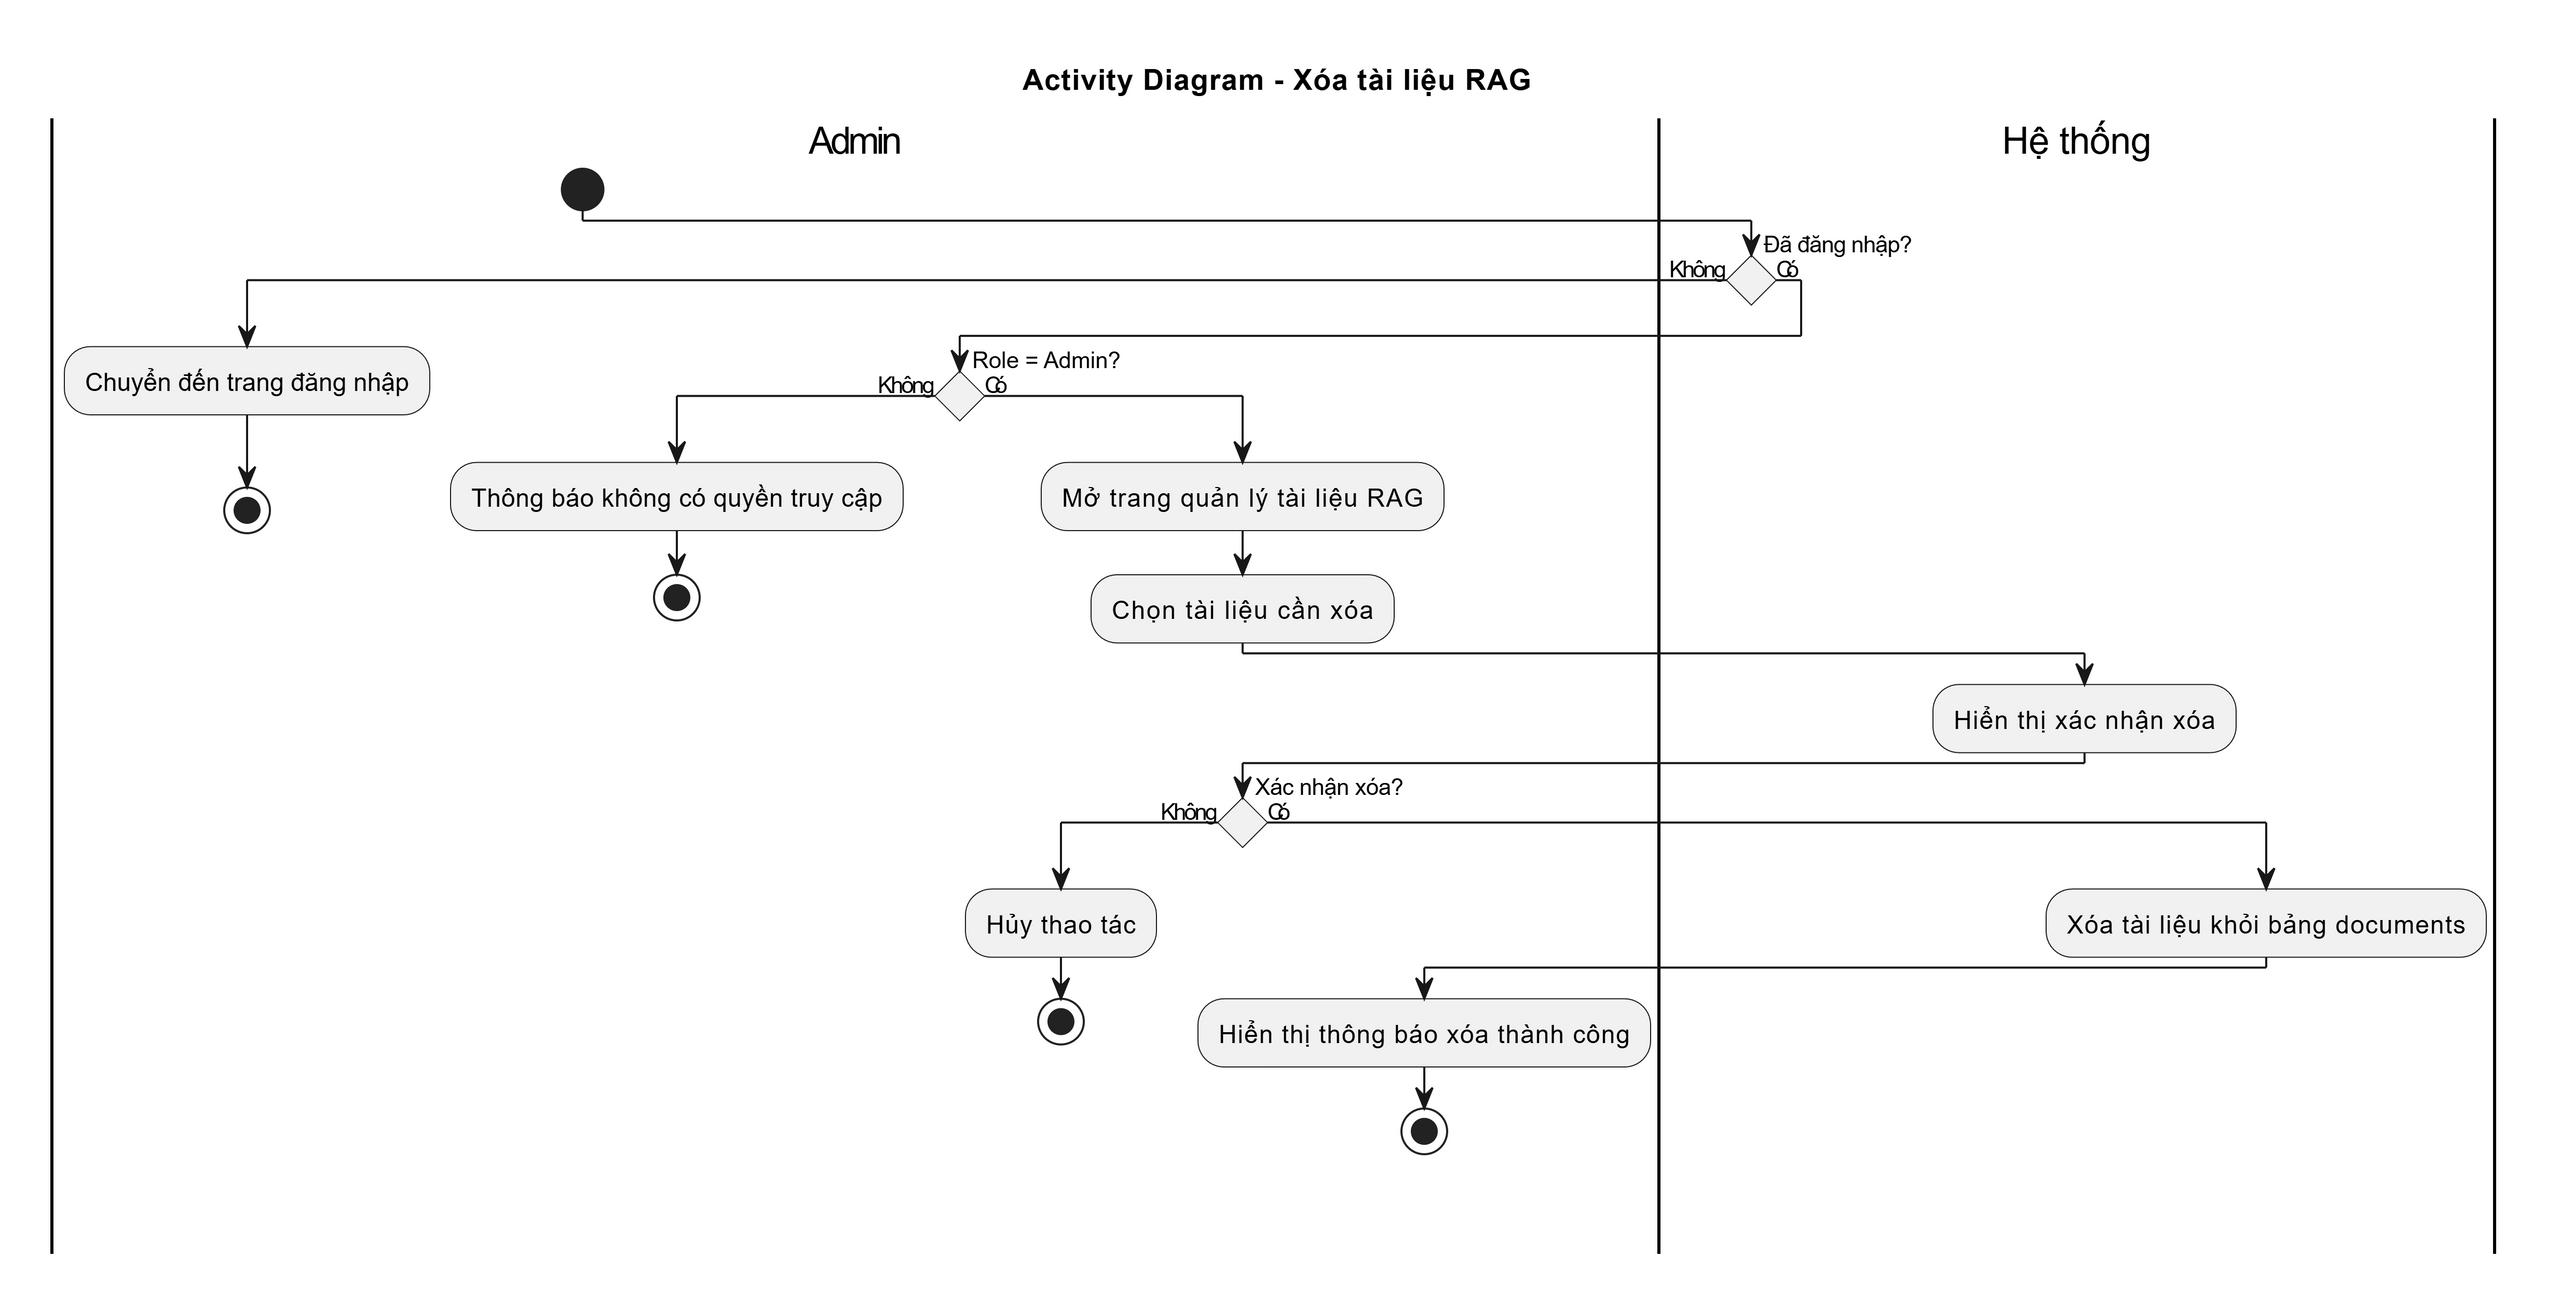
\includegraphics[width=0.8\textwidth]{figures/ac_xoa_rag.jpg}
    \caption{Activity Diagram xóa tài liệu RAG}
    \label{fig:ac_xoa_rag}
\end{figure}
\textbf{Mục đích:} Cho phép Admin xóa tài liệu không còn phù hợp hoặc lỗi thời khỏi Vector Database để duy trì chất lượng dữ liệu cho chatbot RAG.

\textbf{Luồng hoạt động:}

\begin{itemize}
    \item Hệ thống kiểm tra đăng nhập:
    \begin{itemize}
        \item  \textit{Nếu chưa đăng nhập:} Chuyển đến trang đăng nhập và kết thúc.
        \item  \textit{Nếu đã đăng nhập:} Kiểm tra quyền truy cập.
    \end{itemize}
    
    \item Hệ thống kiểm tra Role = Admin:
    \begin{itemize}
        \item  \textit{Nếu không:} Thông báo không có quyền truy cập và kết thúc.
        \item  \textit{Nếu có:} Mở trang quản lý tài liệu RAG.
    \end{itemize}
    
    \item Admin chọn tài liệu cần xóa.
    
    \item Hệ thống hiển thị xác nhận xóa.
    
    \item Admin xác nhận xóa:
    \begin{itemize}
        \item  \textit{Nếu không:} Hủy thao tác và kết thúc.
        \item  \textit{Nếu có:} Xóa tài liệu khỏi bảng documents.
    \end{itemize}
    
    \item Hiển thị thông báo xóa thành công.
    
    \item Kết thúc quy trình.
\end{itemize}
